\documentclass[12pt,openany]{book}

%PACKAGES%
\usepackage[inner=19mm, outer=19mm, top=25.86mm, bottom=25.86mm, papersize={154mm, 216mm}]{geometry}
\usepackage{graphicx}
\usepackage[english]{babel}
\usepackage{fontspec}
\usepackage{enumitem}
\usepackage{sectsty}
\usepackage[]{titlesec}
\usepackage{verse}
\usepackage{fix-cm}%font size
\usepackage{multirow}%tables
\usepackage{array}%tables
\usepackage[hyphens]{url}
\usepackage{tocloft}
\usepackage{soulutf8}
\usepackage{marginnote}
\usepackage{caption}
\usepackage{wrapfig}

\graphicspath{ {./images/} }

\renewcommand*{\marginfont}{\SkolarLight}

%this snippet of code is a bit of a hack to allow line break after em-dash (http://tex.stackexchange.com/questions/62800/lualatex-and-line-breaks-after-em-dashes)
\catcode`\—=13
\protected\def—{\unskip\textemdash\allowbreak}

%\usepackage{pagegrid}
%PACKAGES%
%\pagegridsetup{top-left, step=3.435in}

%TABLE OF CONTENTS%
\renewcommand*{\cfttoctitlefont}{\Secfont\Large}%use tocloft
%TABLE OF CONTENTS%

%LINESPACE% SETS LINESPA\caps{ce}
\usepackage{setspace}
\setstretch{1.15}
%LINESPACE%

%FONTS%
\setmainfont[Numbers=OldStyle]{Alegreya}
\setsansfont[Scale = MatchLowercase]{Alegreya Sans}
\setmonofont{Alegreya}

\newfontfamily\Chapfont[ItalicFont=Alegreya Sans Italic]{Alegreya Sans}
\chapterfont{\Chapfont\LARGE\centering\mdseries\setstretch{1}}
\newfontfamily\Secfont[Numbers=OldStyle]{Alegreya Sans Medium}
\sectionfont{\Secfont\mdseries\large\setstretch{1}}

% Adjust sectional unit title fonts in ToC
\renewcommand{\cftchapfont}{\sffamily}
\renewcommand{\cftsecfont}{\sffamily}

%HEADINGS%

%HEADER%
\usepackage{fancyhdr, textcase}
\setlength{\headheight}{15pt}
\pagestyle{fancy}
\renewcommand{\chaptermark}[1]{\markboth{\thechapter.\ #1}{}}
\renewcommand{\sectionmark}[1]{\markright{\thesection\ #1}}

\fancyhf{}
\fancyhead[CE,CO]{\thepage}
% \fancyhead[CO]{\headcaps{\MakeUppercase{Ajahn Buddhisaro}}}
\renewcommand{\headrulewidth}{0pt}
\fancypagestyle{plain}{ %
\fancyhf{} % remove everything
\renewcommand{\headrulewidth}{0pt}
\renewcommand{\footrulewidth}{0pt}}
\newfontfamily\headcapsfont[RawFeature=+c2sc]{Alegreya}
\newcommand\headcaps[1]{{\headcapsfont #1}}
% \fancyhead[CE]{\headcaps{\MakeUppercase{Presence Awareness}}}
%HEADER%

%HANGING LEFT%
\newcommand*{\vleftofline}[1]{\leavevmode\llap{#1}}
%HANGINGLEFT%

%WIDOWS & ORPHANS%
\widowpenalty=10000
\clubpenalty=10000
%WIDOWS & ORPHANS%

%Applies various subtle improvements in typography. Use default.
\usepackage{microtype}
\frenchspacing

\usepackage[unicode, hidelinks, pdfauthor={Buddhisaro}, pdftitle={Presence Awareness}, pdfsubject={Buddhism}, pdfkeywords={Buddhism, bhikkhu, monks, Sutta, tipitaka, tripitaka, sutra, samatha, vipassana, calm, insight}, pdfproducer={LuaTeX  beta-0.70.1}, pdfcreator={LaTeX2e}]{hyperref}

%DOCUMENT INFO. NOT USED IN TEXT.%
\title{Presence Awareness}
\author{Ajahn Buddhisaro}
\date{}

\begin{document}
\frontmatter
\pagestyle{empty}
\newgeometry{margin=0pt}

\hspace*{-159mm}
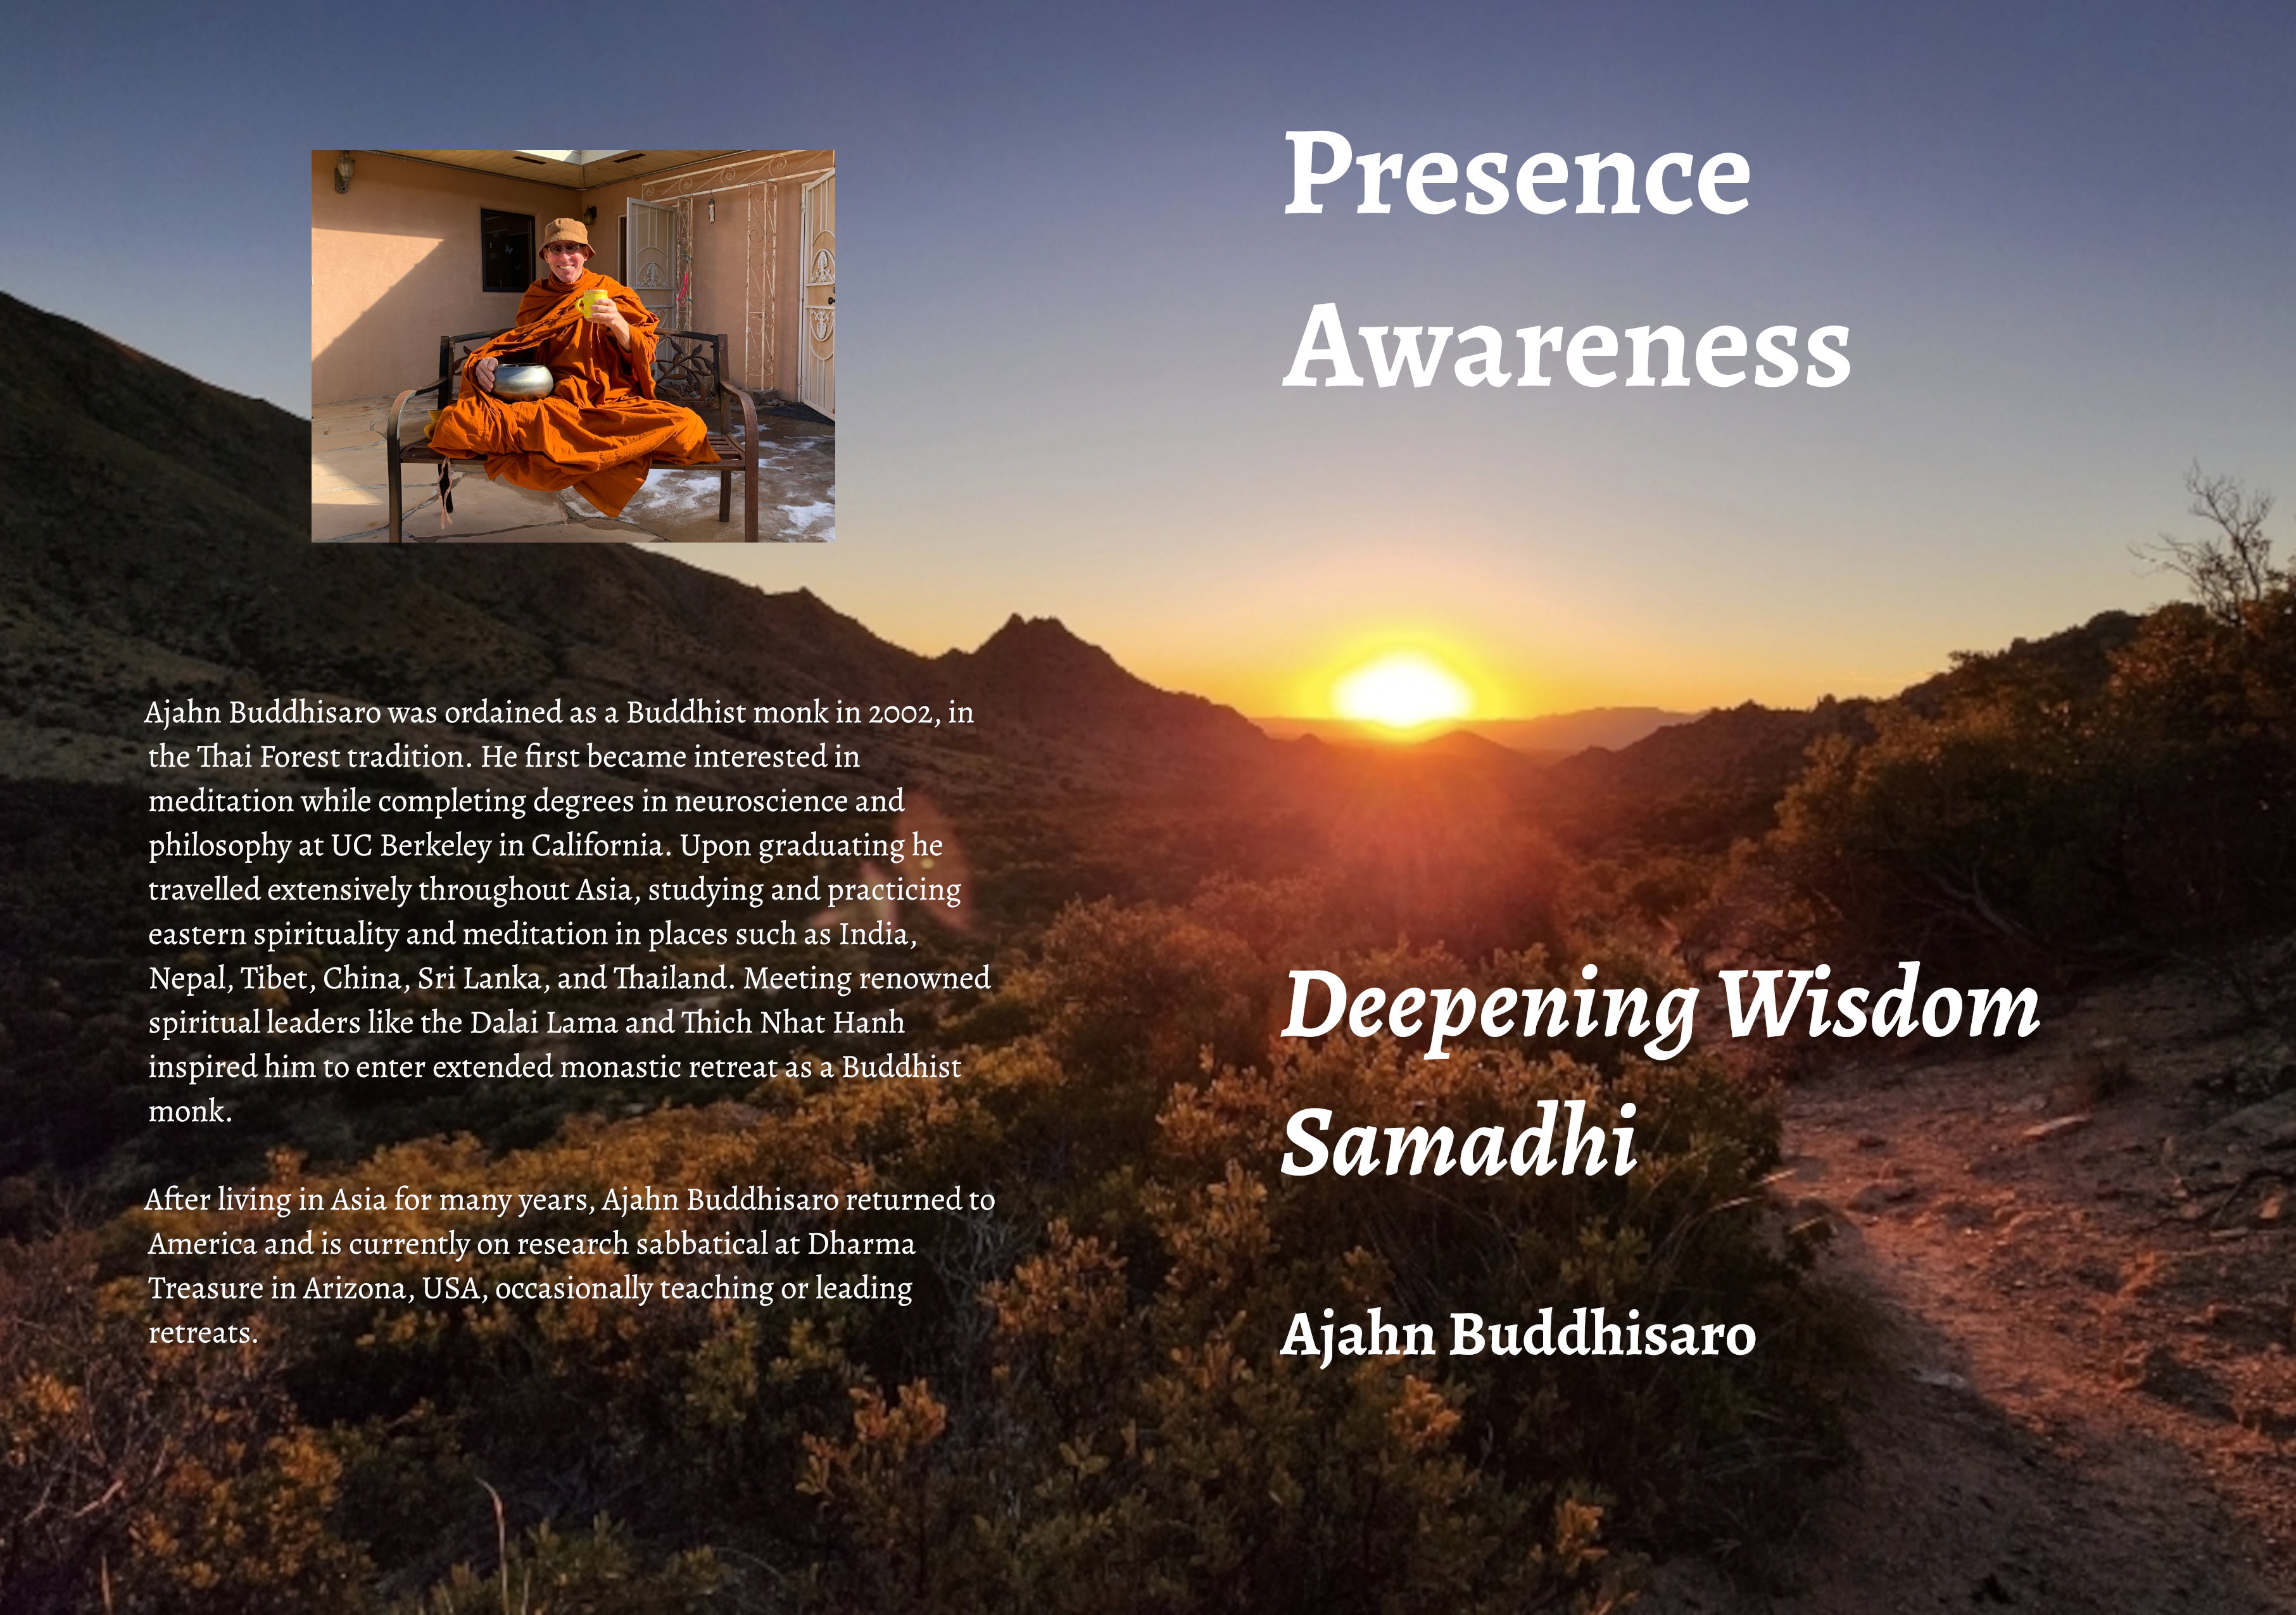
\includegraphics{cover.png}

% \begin{center}\end{center}
% \begin{center}

% \vfill

\maketitle

% \vfill
% \end{center}

\newpage
\restoregeometry

\begin{center}\end{center}

\vspace{4em}
{\small
\noindent Based on a retreat given in September 2023 \\at Dharma Treasure Retreat, Arizona, USA.

\bigskip

\noindent Copyright Ajahn Buddhisaro

}

\vfill

\begin{center}
\textit{May all beings be well and happy!}

\end{center}
\vfill

\newpage

\tableofcontents

\bigskip

\vfill

\begin{figure}[h]
    \centering
    \makebox[0pt]{%
    \includegraphics[width=0.83\paperwidth]{dragoon.jpg}}
    \caption*{Dragoon Mountains \textit{(all photos by Ajahn Buddhisaro)}}
\end{figure}

\vfill

\mainmatter
\chapter*{Awareness Meditation}
\addcontentsline{toc}{chapter}{Awareness Meditation}

\pagestyle{fancy}

\begin{verse}
Just for now \\ 
Take a deep breath, exhale \\ 
Relax, release any tension \\ 
In the body, the mind, emotions \\ 
Reboot, start from scratch \\ 
Shift the mode of operating \\ 
Away from thinking and doing \\ 
Into being and knowing \\ 
Relaxing and letting go \\ 
Pause and settle in 
\end{verse}

\begin{verse}
Now notice the self evident fact of \\ 
Pure knowing, pure awareness \\ 
Pure being, spacious presence \\ 
This dynamic freeness of being \\ 
Feeling your way into it \\ 
Always already right here right now \\ 
Recognizing and abiding in and as \\ 
Spacious knowing presence awareness 
\end{verse}

\newpage

\begin{verse}
Being the knowing, now is the knowing \\ 
Feeling at ease, present, relaxed \\ 
How wonderful and amazing it is \\ 
Recognizing one is always already \\ 
Right here right now present and aware \\ 
Effortless, naturally, free and at ease 
\end{verse}

\begin{verse}
Now give attention to recognizing \\ 
All sensations in consciousness \\ 
Seeing, hearing, touching \\ 
Thinking, feeling, wanting \\ 
Is all a unification in the knowing \\ 
Is a unification in the now \\ 
As if just pure experiencing \\ 
But sensations are ruthlessly changing \\ 
Awareness lets everything come and go \\ 
Sense of self and wanting come and go too \\ 
Ever new, ever now, ever fresh \\ 
In this spontaneous luminous presence \\ 
All these appearances and disappearances \\ 
Everywhere, any time, anywhere, all the time \\ 
But free of grasping, deception, inherently free \\ 
This just this, gain confidence in liberation
\end{verse}

\begin{figure}[h]
    \centering
    \makebox[0pt]{%
    \includegraphics[width=0.25\paperwidth]{sunset.jpg}}
\end{figure}

\chapter*{Presence Awareness}
\addcontentsline{toc}{chapter}{Presence Awareness}

So as mentioned, this technique or approach, it's often referred to as a discovery approach or a pointing out approach. Because essentially it's attempting to evoke in us a recognition of something which is already present. Present in our being, present in our experience, present in any and every experience. Present in any and every being that is a sentient being. So this pointing out is attempting to evoke in us a recognition of this. Whether we consider it a faculty, or a quality, or a feature, it is an intrinsic aspect or nature of this being. This experience of being, and knowing this experience of being. You see how that's quite artistic, in that it’s not really landing anywhere. An observation which stays suspended conceptually, without jumping to conclusions. So we're just inquiring into our direct experience, our immediate experience. The tech term for this is the phenomenology of what we’re experiencing. What can we discern, what can we recognize, and what can we intuit, about this direct experience we're having right now. And about any experience we’re ever having anywhere, anytime.

So we're looking for a fundamental feature of our experience. And what have we discovered, or what are we discovering? Certainly, the fact of knowing. Pause to check, would we be having any experience at all right now, without the knowing of it? This is not an ontological claim, it's an inquiry into our direct experience. So pause for the moment, and set aside the thinking. We don’t need to do thinking to do this. What do we recognize, what do we discern? This fact of knowing which is inherent to any and all experiencing. So simply this, is the beginning, is the gateway, to this recognition, to this style of practice. The fact of knowing is an essential simplicity and brilliance of it.

Actually,  we're all already acquainted, none of us are beginners, we're all familiar with this awareness style of practice. So this is one aspect of the beautiful simplicity of the awareness approaches, that it is a fact of everyone's experience. Regardless if one has ever meditated before, there is the fact of knowing. In principle, it is self- \linebreak evident. There's a saying, as easy as seeing your reflection in a mirror, is this recognition of knowing, of awareness. Although it is true, it is all too true, that it can remain obscured from recognition or discovery, by what? By thinking, and much more besides. But for starters, to keep it simple, an important part or a huge part of the initial recognition, is about either spontaneously or quite deliberately shifting from the thinking into the knowing. Sometimes we call it unhooking from the mind, shifting from the thinking into knowing. How can thinking obscure the knowing, we might wonder, or if it can at all really obscure the knowing? There's a simile, it's said to be like a solar eclipse where the moon eclipses the sun.

Thinking and attention by nature co-create an object, or like to focus on an object. That's their partnership, their companionship. Mind and thinking, thoughts and attention, like to co-create an object. So this shift really requires a radical stepping out of the mind, or as if seeing what’s prior to it. What is in the background, or in the foreground of thinking. Just like with the sound of the cooler right now. We could say silence is the ever present background of sound, if there really is such a thing as absolute silence. Or we could say that silence is the foreground of sound, depending on what we're tuning into, or how we're tuning into it. Silence and stillness, these are often meta\-phors to show a quality of our experience, or a quality of how we're experiencing something in particular, and our relationship to it.

Prior to thinking, conceptualizing, and labeling our experience, it is already full of sensations. However, if we really are prior to the mind, then sensations are yet being elaborated, conceptualized, and contextualized. This is actually a renowned meditation technique in itself called the Teachings to Bahiya. In the early Pali discourses, \linebreak Bahiya was foremost in being quickest to realize full freedom and awakening. These were the direct pointing out instructions he \linebreak received from the Buddha right there on the spot. In the seeing just the seeing. In the hearing just the hearing. In the sensing just the sensing. And, in the cognizing just the cognizing. And in this space of pure experiencing where it has yet to land on a subject or an object, or reify a relationship between the two, in this space a freedom can be discovered, realized, and awakened to. This is another brilliant essential feature and genius inherent in the awareness approach.

For the recognition or discovery to actually happen, what is required? A subsiding or a meltdown of reifying a subject. A subsiding or a meltdown of reifying an object. What is it that is at the energetic root of reifying a subject object separation and duality out of pure experiencing? This sense of an independent entity on both sides of the equation, which is necessarily overlooking the co-creation and unification principles. We are overlooking the subtle dynamics doing the behind the scenes cocreation, as it were. According to the Buddha, it’s our ignorance and unawareness of that process, and the grasping and the clinging which initiate with it, which are obscuring awakening.

So this realization shift, from the thinking into the knowing, has the potential, or in some sense requires, that that grip of reification subside, loosen, relax, release, let go. That is one very common, very direct way, that this awareness practice actually has inherent insight and realization in it. Because for that shift to happen, the grasping needs to subside, the mental assertion of the me and the mine needs to subside. And in that release one can open up into the space of awareness, or simply the now is the knowing. And from that vantage point it can actually show us that the co-creation of experience is a process. That is a liberation empowerment. That already brings a certain sense of freedom with it, an option for freedom. 

The important thing along with the  co-creation discernment is to be able to see what we've been calling grasping and clinging. That energetic, often very emotional component which compels us to be perceiving things in a certain way. In the relaxation of that, we're free, we’re more free, to reevaluate what we're experiencing and even explore more radical reinterpretations. For that to happen, the tight grip on our preconceived way of experiencing needs to relax. That's why, that's one reason why, relaxation is such an important part of this practice, which perhaps obviously also has so much potential for insight. Relaxation, again, it's like releasing the grip. Just taking a step back that much can show how much sense of self, insecurity, anxiety, and ambition can be fueling all the striving. The Buddha calls it the craving of becoming, becoming. A sense of discontentment, desire and aversion, driving the self ambition ever forward. Perhaps this is too basic for us as intermediate practitioners, but there's usually more subtle insights to be had regarding what the underlying co-creation principles and forces are.

So, in addition to shifting into a natural \textit{samādhi} state, which is aware, which is ever present, which is unshakable, undistrac\-ta\-ble, a pure refuge, remarkably still, calm, bright, alert, and aware. In addition to that, we are getting insight and discernment into how this very fundamental reification of subject and object comes into being. Also how the sense of self bound up with ambitions and agendas is primarily coming from a lot of preconditioned programming and conditioning. These are huge insights as well, because they can free us from being compelled to believe and act in the ways which we've been conditioned to believe and act. We have options to intervene because it's a co-creation event.

So, many of these reflections are designed to open us up, to loosen up or let go of preconceptions and explore new paradigms. The awareness practice is brilliant in this way, in its simplicity and fundamentality. Awareness is not a state we have to create, it's not a conditioned state. We don't have to create it, we don't have to maintain it, and we don't have to lose it. It's really recognizing that it's always already present and aware in this now is the knowing. That recognition itself very much encourages or requires us to pause, at least for now, our reliance on the mind to explain things. What does knowing tell us when allowed to speak for itself? We must initially pause the mind's habitual tendencies of manipulating circumstances, towards improving and optimizing, minimizing and avoiding, pause all of that.

So how to be free from the manipulating tendencies of the mind? That is a superpower. Along with recognizing the knowing, we're \linebreak learning how to loosen the mental grip and set the mind free. We may discover there is a pure contentment also always already available here and now. Just the simple ease of being and contentment, when that engine of desire, craving, and discontentment comes to stillness. This is likewise a promise and guarantee of the Buddha, emerging as a revelation and discovery of the pure contentment refuge. How much of that energy driving becoming is because of an underlying feeling of discontent? Never enough, never good enough, could be better, need to improve, all of that. To at least have an option for refuge in pure contentment. The discovery, oh my gosh, this dimension of pure being, pure knowing, pure contentment, pure at ease, which is inherent in the nature of this being, the nature of this knowing. And that is only the tip of the iceberg. The amount of time, energy, mental energy, emotional energy, and precious resources we're utilizing because we're being driven, compelled, and goaded by that fundamental discontentment. Our precious resources could be used in a much more functional way, for our well being, and to serve the well being of others, it's a guarantee. As we say, bringing evermore wellbeing into being for the well being of beings.

That is no utopian vision, it's a fact of this reality right here right now. This pure being knowing freedom is just waiting to be discovered and realized, but we must be interested. They say it is the birth\-right of all of us, as it's always already in any and every experience we're having, and inherent in the very fact of experiencing itself. But if we are not interested, we may simply continue to overlook it. If we're not somehow dissatisfied, disenchanted, and disillusioned with the old way, then it's unlikely we'll really pay attention and act on it. We must rebel against our mundane mainstream conditioning, all this superficial, unsatisfying,  self image and self ambition story we're playing. If we are not quite dissatisfied with that, outright disenchanted and disillusioned even, we may not have the motivation or the courage to really inquire into this radical new paradigm way of being. Being the knowing.

To put it a bit more bluntly, it’s a shame, it's tragic, and one can't help but feel heartbroken or overwhelmed with sadness. How much unnecessary or avoidable suffering we humans have to go through because of our ignorance. By not knowing and not understanding the reality of our identity, misguided actions often prevail and cause great harm and suffering to self and others, just have a look around. Without clearly discerning how dysfunctional that discontentment driven self ambition conditioning is,  we are stuck repeating the same mistakes over and over and suffering accordingly. That can be heartbreaking. That is heartbreaking. It is the great compassion of the Buddha and the Dharma, the wholehearted aspiration to liberate beings from suffering. There is a way, and this is a very direct way, it's a guarantee.

This and allied approaches are often called direct path or reality path approaches, because they're pointing us to discover a fact of reality that's already self-evident. Or let's say it has a self evidentness to it, meaning it can speak for itself. And the influence this identity realization has on our citta speaks for itself. One feels real and free, feeling free and at ease, the citta feeling in harmony with its own nature, with the nature. So, often they say this first recognition is, as it were, a rediscovery. Sometimes they even call it re-enlightenment, although that's more just a catchy phrase. But it points to this aspect of just our pure knowing nature recognizing or discovering itself, it's as if a recognition of itself. And that's enough to break the spell, the hypnosis, of being identified as a conditioned self, a body mind consciousness sense of self.

Consider, where does that body mind consciousness self of sense arise? We can see this body, this is my body, and I can see it. Is that not an object in my knowing? The body is an object in my seeing, in my touching, in my sensing, and hence it's an object in the knowing. Well, it can't be entirely the knowing in itself, because sometimes the knowing is knowing other things unrelated to the body. So the body, my body, arises in the knowing. Now take this mind, if there is such a thing called mind, this inner activity of thoughts and thinking. Say to yourself once, whatever your name is, say I am Buddhisaro. If we say it silently inside, we may hear it, or we may see it, like a ticker tape. Thoughts, they’re like ticker tapes. That thought isn't me, and it's not only the knowing either. The knowing seems to be itself regardless of the content, and all the objects of knowing seem to be the content. And the content is always changing, appearing and disappearing, in small ways and very big ways. So look, everything we can witness in the knowing is a sense object of or in consciousness. But the knowing itself is simply the knowing.

So this can be a legitimate first step in shifting into the knowing, just to explore that distinction between the knowing itself and the content of knowing. See how the content is always changing. In fact it seems sense consciousness has to work this way, sensations have to change to be perceived. If sensations stop changing, they drop out of consciousness, as it were. So without jumping to conclusions, we can inquire into what is the least changeful aspect of our experience? Or we may as well say what is the most changeless aspect of our experience? This inquiry, when successful, highlights the contrast between the pure knowing and everything else which is changing. The Buddha proposed impermanence and dependent origination as supreme insight themes for deconstructing the habits of subject object reification, and consequently releasing the grasping and suffering. As they say, the fact of it is, we inquire into  suffering and find inevitably that it is not being in harmony with the nature of the way things are.

So this is not just adopting a new view or a new belief, but it's an attempt to discern a more fundamental reality of the way things are. So it requires us to look and see for ourselves. To the extent we're more stubborn or skeptical, we will require more convincing and evidence. Try to stop a sensation from changing, right now. It's easy to see with speech or with sound. With speech, one syllable has to yield to the next, and one word has to yield to the next, and sentences likewise, so with speech it's quite easy to see. Sound, we notice fluctuation, which is evident in change. The spinning fan, things in motion, that's also easy to see. The physical and tactile sensations we're feeling, they vibrate, or we even see our attention shifting from one sensation to another. Well that's change. What if anything, what in our sensory experience is not changing?

Well, certainly from the vantage point of the now and the knowing, every sensation must be changing. Change implies time, the \linebreak phase of appearing and the phase of disappearing. From the vantage point of the now and the knowing though, all sensations seem ruthlessly transient, as if by nature. That insight, that realization, can't help but release the grip of reification and grasping. The insistence that they don't change when they do, and the insistence that they do change when they don't. And hence shifting into a more harmonious flow state, with the flow of appearances and disappearances, which are simply acting quite in accordance with their own nature. As co- \linebreak creation co-arising, and codependent co-ceasing phenomena of experiencing. 

This is all self-evident from the vantage point of the knowing, of the now is the knowing. And the sense of the person, the selfhood, the story, that's all a part of the flow of events, the flow of sensations. See, it's really taking a step back into this bigger picture to hold the space of the totality of experiencing. Any and every sensation, any and every experience, has this cocreation knowing as its fundamental nature. That is a revelatory insight, when we shift into harmony and alignment with it. It can not help but release the reification and grasping, the clinging to archaic views we have about what we're experiencing. 

So, there is much more to be discovered, much more to be said. We'll have a Q\&A this afternoon. We can start one on one sessions tomorrow afternoon maybe. Today we’ll just get settled in, and get clear about what some of our clarity or confusions are. And hopefully we’re directly experiencing how integrated this really is, our understanding about what we’re experiencing, and how that can initiate a lot of shift into the knowing. Through insight, through emotional release, and through energetic relaxa\-tion. It really is one whole event happening, and this awareness approach exploits that, the unification principles. So please aspire to be earnest and to persevere, and there will be great benefit, it’s a guarantee.

\chapter*{Flow State of Knowing}
\addcontentsline{toc}{chapter}{Flow State of Knowing}

Okay, for those of us who already know how to drop right into the meditation, or we're already in the groove, just drop right in. See, that’s a technique in itself. To bypass steps, to bypass stages, and just drop right in. Or maybe we've yet left our meditation since the last session even. We’ve been able to keep our continuity, according to our aspirations. It can be so.

And see, part of the technique here is, it's actually called the recognition or the discovery approach. It's the recognition or the discovery that awareness or knowing is always already right here right now. The technique for dropping into it is simply recognizing that. Maybe we hold back a bit, because we become familiar with following steps and stages. See if one can simply set that aside, and drop right in. It's like dropping into a flow state. The knowing, it's always now, and now, and now.

If the drop is too abrupt, then do a sweet little three step drop. Settle the body, and relax the body. Settle the breath. See that you're feeling loose and natural, belly breathing yet  naturally. Relaxing the face is very important for this practice. It has a direct effect on the mind. Soften the gaze. Eyes open is very important for this practice as well. We're greatly encouraged to experiment with this as an eyes open meditation retreat. Ajahn Chah notoriously said wisdom arises on contact, and we practice with our eyes open. And this is a wisdom awareness retreat. We’re calling it wisdom \textit{samādhi}, which will become more clear as we go along.

So step one, relax the body. Step two, relax the mind. In a very similar way, just invite the mind  to be open. Invite the mind to be free of thoughts and concerns of the past, thoughts or concerns about the future, and any thoughts or concerns about the present. Everything is perfect right now. So similar to that subtle relaxation intent when sweeping through the body, and you feel some tension or contraction, and you can release it. Do just that kind of sweeping your awareness with relaxation intent through the mind. 

Sometimes it helps to do a little mental exhale, as it were. Not forceful, but just releasing, like opening the hand. It's not necessarily a letting go, it’s just relaxing the grip and releasing. No need to think about anything, just set the mind wide open and carefree. It doesn’t need to get concentrated, and it doesn’t need to fight with distraction. Our mind is just free to be open and carefree. 

Step one, relax the body. Step two, relax the mind. Step three, drop right in. Maybe as an aside or a footnote, one could have a confident intention to keep this continuity of knowing, clear and lucid, for the full duration of this meditation session. And that doesn't mean striving or micromanaging, it means entering into a flow state of knowing. And staying there and being that. Being the knowing.

Now and then, or as needed, if it starts to space out or slip a little, just brighten up. Just refresh, refresh the knowing, refresh the sense of now, but without making a fuss about it. Just refresh, keep it fresh, cruising right along in that flow state, the flow state of knowing.

If it's too formless, you can have a little internal mantra, like \linebreak maybe now is the knowing. The great reminder, now is the knowing. Now is the knowing. Ever new, ever now, ever fresh, now is the knowing. Or perhaps the mantra, always already present and aware. Where? Right here. When? Always now, now, now. Always already present and aware.

If we start seeing lights, that's fine. Just stay with the knowing, stay in the flow state. If we feel energies, that's fine. Stay with the knowing, stay in the flow state. This flow state in the knowing, it does not get hooked by sounds, by sensations, or by thoughts. Anything and everything just flows right through the knowing, the awareness. Awareness and its inherent unconditional love. It lets anything and everything arise into the knowing, and it lets anything and everything pass out of the knowing, according to its nature. That is the nature of the knowing, in the flow state of the knowing.

Check in. Are we still here, right here right now? Now is the knowing. Timelessness, the timeless now. We've got to think to make time, otherwise it’s always now, and now, and now. Keep it fresh, but not too tight, not too loose. Alert, awake, and aware. Deeply relaxed and content, and carefree. Go ahead, see if you can enter \textit{samādhi} using the knowing.

If it's slipping or getting spacy, then refresh and revive. Open your eyes, incline your gaze a bit. Revitalize your posture. Energize your mind. And become even more adept at countering the slippage or spaciness before it takes hold. Keep it fresh. This is not for sloppy meditators.

With your eyes open, it can help to fix the gaze on whatever object the gaze happens to meet. Without focusing much at all, just let the gaze rest on whatever object that might be. Let the gaze rest. Steady the gaze, and see how it has a direct influence to help still the mind. Are you seeing that? Stay with it for a few minutes.

It’s very important to relax the gaze, and just let it rest there. This is only to fix the gaze, not to focus the attention. Notice that if the gaze tends to slip, the mind tends to move, and if the mind tends to move, the gaze tends to slip. Make a special note of that. This is a protip to steady the mind doing eyes open meditation. Keep it fresh. 

We are indeed developing new skills, right now. Your earnestness and perseverance will bear fruit, guaranteed. Continuity of knowing, flow state of knowing. Pure and simple, one task, being the knowing.

If it seems like it's requiring too much intention, experiment with easing up just a little bit. Just ease up on the intention, or ease up on the attention. Ease up a little bit, and just see if you can still be with the knowing.

Now we're feeling a little more relaxed and at ease. Because too much effort with intention or attention can cause energy deficit. So we want to use the very minimal amount required. We can see if our meditation were to shift into being the knowing, how effortless that would be. How much effort does it take to be what you are? You are what you are, always already. 

Likewise, if it feels a little too loose, or a little too spacey, a little too slippy, well then refresh and revive, and revitalize the knowing. It’s finding that balance of not too tight, not too loose. Completely awake and aware, yet deeply relaxed and at ease. The supreme remedy for both restlessness and dullness, the major challenges for advanced meditators like us.

As well, it's fine if the pure knowing seems a bit too subtle and sublime for us right now, try knowing hearing. Like the crickets in the distance, what a lovely sound. While hearing the sound of the crickets, be aware of knowing hearing. Am I hearing the crickets? Why, yes I am. But how do I know? Why, through knowing hearing, knowing hearing. In this way, one can be in the flow state of knowing through knowing hearing. When? Well, now is the knowing, knowing hearing. And in the very same way one needs to keep it fresh, keep it fresh. 

Every now and then taking a few deep belly breaths can be very refreshing as well. Knowing breathing, knowing breathing. When? Now, now is the knowing. Likewise, if it doesn’t feel like it’s disrupting our continuity, we can just sweep a relaxation through the body, and see if any tensions or contractions have arisen. Sweep a relaxation through the mind, and release any arisen stagnation or tension. We can even do a global scan of awareness through each of our six senses, to refresh the clarity of the knowing. And then drop right back into stillness, into now is the knowing. Now, and now, and now. Keep it fresh, keep it fresh. Ever new, ever now, ever fresh. Now is the knowing.

Watch the past and future drop away. Watch the timeless now emerge and reveal itself, in all its glory. Let the mind and awareness come to stillness in unification, unification \textit{samādhi}. Things are very different than we think they are. Knowing hearing. Now is the knowing. Being the knowing. Everything is arising in the knowing. The knowing and the sensations are not two things, feel free to let them unify according to their nature.

Keep a check to see you are completely relaxed. See if you can let go paying attention altogether while still remaining aware. No striving is involved, just releasing intentions, releasing attention. When conditions are right, it will unify all on its own. Watch where the sense of self goes. Where does it emerge from and where does it return to? What is the source of subjectivity? No mental intentions, no bodily tensions. Pure stillness and relaxation. The nature of awareness. Now is the knowing. 

When it's challenging to keep it fresh, and we persevere to keep it fresh, that's when our meditation practice is developing. Please be earnest, please persevere to keep it fresh. That's the cultivation we're looking for, that's why we're here. Keep it fresh. Your earnestness and perseverance will bear fruits, it's a guarantee. 

May all auspicious circumstances prevail, may our highest aspirations be fulfilled. 

\textit{Nibbānassa paccayo hotu, nibbānaṁ paramaṁ sukhaṁ, svaha svaha svaha.}

Ok, we wish everyone a good night and good practice.

\medskip

\begin{figure}[h]
    \centering
    \makebox[0pt]{%
    \includegraphics[width=0.6\paperwidth]{clouds.jpg}}
\end{figure}

\chapter*{Wisdom \textit{Samādhi}}
\addcontentsline{toc}{chapter}{Wisdom \textit{Samādhi}}

So, it's important with the wisdom \textit{samādhi} practice, or for wisdom \textit{samādhi} to arise, that we carry our insights with us all the time. And that we carry our meditation, our sati, our \textit{samādhi}, our equipoise, with us all the time. For instance, during the sit this morning, or since the retreat began even, if there is a particular insight theme or insight object which is resonating with us, we are becoming familiar with suspending our awareness and attention to encompass that theme. Not really landing on it as an object, but just sort of embracing its manifestation in experience, or as its manifesting. See, that’s the thing about these kinds of insights, they're actually just recognizing aspects or qualities of nature that we're experiencing right now. Right now, anytime and every time. Here, anywhere and everywhere. That's the nature of a universal insight, of a Dharma insight. It's intrinsic to our nature and what we're experiencing, always.

So whatever retreat realization theme we're resonating with,  and taking as our wisdom \textit{samādhi} object. Or perhaps we already have a prior theme of insight we're familiar with and inspired by, and feel a karmic connection to, and are using that. Maybe a wisdom theme was transmitted to us from a beloved teacher, or a beloved teaching was just exceptionally fresh and inspiring for us in the beginning \linebreak while we were initially discovering the Dharma. Whatever the case may be, we're becoming more familiar with suspending that realization theme within the actual feeling of the insight event. That sense of aha, that realization, that eureka, that novelty of the insight realization event. That exhilaration of novel understanding and seeing clearly the nature of things. The intuitive, unmediated knowing \linebreak which arises inside as if from our own heart, liberating it from the ignorance of not knowing. It is completely prior to thinking or conceptualizing or analyzing, as if making an independent, self-evident assertion of its own, just expressing or proclaiming the nature of nature.

So, that feeling of revelation, or exaltation, the newness, the freshness. We want to have that liveliness in real time of the genuine insight itself, not as memory of past experiences. It is alive, it's happening right now, and the heart's realization of it is happening right now. That's that fresh revelation and liberation sense of the insight. That's when we know it's gone beyond the mind, behind the mind, or through the mind, into the heart, into the citta. That's what we’re intent on here and on the lookout for, that taste of freedom. The \textit{vi\-mut\-ti ra\-sa}, that sense of freedom, that taste of freedom. Every insight of the Dharma has the taste of freedom. It's liberating, it's freeing us, freeing us from the ignorance, from the unawareness, from the not knowing. Something we didn't know before has been revealed or discovered or recognized, and the ignorance of it vanishes on the spot. Like the simile of darkness in a cave. It matters not how long darkness has been in a dark cave, for as soon as the lantern is lit, it is flooded with light. That is the light, the aloka, the light of awareness, the light of wisdom, the light which dispels the darkness of ignorance. Like the dawning of the sun rising to dispel the night. The sun knows not darkness. One who spins with the earth necessarily knows day and night, but one who stays with the sun knows not darkness.

That's the transmission nature of the realization event. It has the \textit{vi\-mut\-ti ra\-sa}, the taste of freedom. Freeing the heart and mind from ignorance, from confusion, and from misunderstanding. For so long it has been misled and misguided, perhaps all very innocently so. \linebreak There’s a saying, ignorance is innocent like a child, because it doesn't know for itself, it's just learning what it’s being taught. Ignorance is innocent, it’s not the villain here. It’s like an innocent child, it needs nurture, to grow, to develop, to become wise and self reliant.

The \textit{vi\-mut\-ti ra\-sa}, the taste of freedom. What is coincident with a deep insight, what is coincident with a realization event? The ignorance subsiding initiates the releasing of grasping, the releasing of clinging, and in effect the releasing of the grip of the me and the mine. And to that extent, it results in the relaxation of desires and aversions of any and every kind. And that great sense of relaxation and relief, that the moment is being redeemed, harmony is being restored, and we’re returning to an alignment, a being in harmony with the nature of the way things are. This is the promise of the Buddha, and this is the guarantee of the Dharma, and of fruitful Dharma practice. If one is earnest and persevering, it is a guarantee that correct practice will be of great fruit and great benefit.

So, very important for developing in the wisdom \textit{samādhi} practice is paying special attention to the transitions, the interim between sessions. When we’re changing postures and activities, such as rising from the morning sit to go for a walk, pause to recheck and reestablish your sense of knowing, your sense of \textit{samādhi}, and with having your insight theme clear. And then in a very natural way entering into this flow state of wisdom \textit{samādhi}, this is the way of practice. So very naturally staying tuned in to the sati, to the \textit{samādhi}, to the wisdom theme, and to the intention aspiring for fruitful practice. We’re only here for seven days on this retreat, but one privilege of being on retreat is that you can intend for virtually 24/7 practice throughout. Although that will only happen if you've higher inspiration, priority, and a sense of urgency, and it’s quite meaningful to you in this way.

Often to begin a retreat, as we know, there's a whole topic devoted to arousing the intention, the aspiration, the priority, the sense of urgency, the resolve, and the group energy to be fulfilling the intention and aspiration of the retreat. So, usually there's a whole topic devoted to that, so we can be crystal clear of our intentions, and have that as our foundation for practice. This great aspiration for spiritual realization and service actually matures into an ever present benevolent energy and unified intent that we as sincere practitioners carry with us all the time. To a large extent it is uncompromising regarding its clarity of purpose and decision, aspiring to bring about spiritual fulfillment in any and all situations. When quite mature, it rarely doubts or hesitates in action, and remains true, loyal, and in alignment with what those Dharma intentions and priorities are. Of course we know that this is one way of speaking about the noble eightfold path as it develops in a unified way. Integrating all our activities of body, speech, and mind throughout the day, within this unified intent to actualize the Dharma. To have all our intentions and actions be wholesome, be skilful, be beneficial, and in alignment with the Dharma. It is really so important. We’ve just touched on it here briefly because it's presumably a prerequisite for intermediate practitioners, and somewhat familiar and well established in us already. 

So we start with stabilizing and deepening our wisdom \textit{samādhi} on the cushion. Now before concluding our session, we pause, If only for an instant, to do an internal check in, a reality check, that during the transition we will remain in meditation while proceeding to the next activity, and into the next session. It's fine however often we need to check in and do this, like connecting the dots, to just reestablish our intent for continuity. Just check in, like with a mindfulness refresh, like we've been doing during the sitting sessions. Just refresh, check in, reestablish your sati, reestablish your \textit{samādhi}, and reclarify your wisdom or insight theme. Just like we're doing with the eye gazing in the meditation, and we can see when things go a little fuzzy, or slip a little bit. Just refresh, reclarify, and reestablish our practice with balanced intent and equipoise. We want to get in the habit of doing that often and all throughout the day for integrity and continuity of practice to arise. That's what they say, at first our commitments and efforts are sporadic and haphazard, and then recur more frequently. Then they become more stable and consistent, and finally are continuous and intense. When our inspiring practice is consistently deep, clear, stable, and continuous, this is the most opportune time for realizations and breakthroughs to be happening. Continuity and clarity, being free from doubt and hesitation, and being with unified intent. These are optimizing conditions for realizations to clarify and go deeper, and inevitably translate into action. 

So regarding our wisdom \textit{samādhi} realization theme, say for example we’re really connecting or resonating with the theme of the now, today’s theme of the now. Or perhaps even for quite some time already we've been inspired by the now theme, like the power of now. To have that insight really bear fruit as wisdom \textit{samādhi}, we're not simply just abiding in the now, but we’re seeing what are the implications of this. What are the implications of the now realization? Like in our guided meditation this morning, knowing from the vantage point of the now, what does that teach us about experience, about sensations, about grasping? Where are all the experiences now, all the delighting and enjoying, all the worry, pain, and suffering, of the past ten, twenty, thirty, forty years or more? Where are they now? All of the story, the history, the personal narrative, where are all those memories of experiences now? Imagine if we died yesterday, just \linebreak pause a moment to contemplate that. How much do we actually remember from the past twenty or thirty years, and where's all that experience that's unremembered? Can memory even stand up to an actual experience, when it’s seen to be simply a mental activity happening in the mind, in the now? How will any future experiences turn out to be otherwise? So from the vantage point of the knowing in the now, or the insight wisdom theme of the now, one’s getting deeper realization into the actual nature of experience itself. One can't help but be getting deeper insights into the nature of sensations, into the nature of significance, the nature of desires and aversions, into the nature of the personal sense of self. All of that is experiencing actually transient to the now. We only call it a genuine wisdom realization when the insight goes deep enough to speak for itself, actually revealing some aspect of reality, the nature of the way things are, and most importantly knowing clearly what the implications of that are for liberation. So whatever ignorance gets liberated and subsides, to that extent grasping is subsiding, and to that extent there’s suffering subsiding. We are more in harmony with the way things are, and to that extent we are free from ignorance and suffering. 

Or again, regarding our wisdom \textit{samādhi} realization theme, take for example the pure knowing, or the pure awareness. It's not enough to be simply abiding in the knowing awareness. That’s actually not sufficient for wisdom \textit{samādhi} or genuine insight to arise. In fact, it's still considered just a \textit{samatha} or \textit{samādhi} practice by the wisdom traditions, which doesn't necessarily yield liberating realization. But as we've been mentioning, the awareness practice is brilliant and genius in many ways, and is one of the foremost ways for developing wisdom \textit{samādhi}. Inherent in the very nature of the knowing awareness, or more precisely the pure knowing and pure awareness, is the nonself emptiness insight,  the sense of being free from the me and the mine. Pure knowing is inherently free from grasping. Pure awareness lets everything come and lets everything go. Even this element of unconditional love and unconditional acceptance is intrinsic in pure awareness, which itself doesn't say this is me and mine. That I making and mine making is an activity of mental formations, it's a process of mental fabrications. Look, that sense of selfing is a ripple in the mind. Don't we need memory to have a me and a mine? What is this me and mine that that's actually referring to? Oh, of course, it's my experiencing, my feeling, my perceptions, and my memories. It's my desire, my fear, my aversion, my love, and my hate. All this me and mine, well awareness doesn't say that. Awareness is pure, free, open, expansive, all pervading, all encompassing, pure knowing by nature. And it is self evident, it speaks for itself, the sense of emptiness, the sense of nonself. The supreme nonself emptiness realization insight of wisdom \textit{samādhi}. See, that's not just knowing. One could walk around all day saying me and my knowing, me and my knowing, me and my presence awareness. But that's from the point of view of the mind which is naturally just doing its thing of I making and mine making. It’s in the nature of the ignorant mind to appropriate everything as an object, and make it into a me and a mine. To substantiate or reify the subject and the object to make it into a me and a mine. It’s the nature of sankhara, when it has avijja ignorance as its puppeteer, to be a virtual magician at making everything into me and mine. And that is certainly the magic of the mind, and we do not dismiss it. After all, it is co-creating everything we're experiencing. We are just looking to get deeper insight into it, to see through it, to discern what the underlying first principles are, or as close as we can get. What is the reality of our experiencing right now?

So, another example realization theme for wisdom \textit{samādhi} is sensory consciousness. What if the retreat insight theme which is resonating is sensory consciousness, like knowing seeing and knowing hearing. What are the implications of everything, all sensations in consciousness arising in the knowing? Nothing can be separated \linebreak from the knowing, in direct experience that is. With intellectual abstraction or philosophy, or through imagination or whatever, we can contemplate knowing in many ways, but in our direct experience we see that we cannot separate the sensation or the experiencing from the knowing of it. Like the beautiful granite dome up there, and the bright blue sky. Where are we experiencing that, out there or over there? In here or over here? See, there's a sense where the inner and the outer begin to unify in the knowing. Wherever there’s consciousness, there is knowing. Wherever there’s a sensation, even as subtle as space, there is knowing. What are the implications of that? Our naive sense of a me in here and a world out there, and the separation inherent between the two. What are the implications of that, and what is the insight into the co-creation event? What does that insight do to the separate sense of self, and what does it do to the separate sense of others? What does it do to the sense of being the victim of circumstances, and what does it do to feeling the need to manipulate circumstances? How does that insight impact on overlooking the flow state, what does it do? What do the insights do, and how do they transform our meditation into wisdom \textit{samādhi}? We want to be getting more and more clear on it.

So we see, on this retreat we are focusing on several wisdom \textit{sa\-mā\-dhi} realization themes and they're all overlapping. They're all speaking to the fact of knowing our direct experience, and realizing the co-creation nonself emptiness dynamics which would seem to be self-evident structures of its nature. And these, among others, are primary insights the Buddha is pointing to, to free us from ignorance and grasping, and a way of being in harmony with the nature of the way things are. Being free from craving, one feels peaceful, at ease, and in harmony, but it's through discerning the underlying reality principles. The Buddha called these three primary insight themes the three doors to the deathless, the gateways to \textit{nibbāna}. The nonself emptiness realization. The impermanence and changeability realization. The desireless free from grasping and clinging realization. The Buddha emphatically instructed us with these three celebrated wisdom \textit{samādhi} doors to the deathless.

So keep the theme of insight fresh, and keep seeing what the implications are. How is it relevant in real time, and what is the effect of this insight on my understanding of what’s happening right now? What influence does it have on my grasping, my reactivity to experience, my relationship to experience? How am I feeling the freedom and the sense of ease, and bringing that to the forefront. That's how we gain confidence in the fruitfulness and efficacy of the insight realization to deliver its promise of freeing the heart and mind from ignorance, from grasping, and from suffering. Or in the more positive sense, we're gaining confidence and conviction in the bliss, the sense of ease, the peace, the reverence and appreciation, the unconditional love and acceptance, the feeling in harmony with the nature of the way things are.

So please be clear about this. Maybe the homework for the day is to check in and see which insight theme seems to be most relevant, and that you already have the most confidence in, and holding that as your mindfulness reflection throughout the day. If you’re already able to be more clear and stable with it, then take it as your wisdom \textit{samādhi} object. And throughout the day, keep seeing the implications of the insight in real time. What power does this insight have to assert the sense of being free, the taste of freedom and liberation. What power does it bestow towards feeling more in the harmonious flow state of knowing, in the flow state of wisdom \textit{samādhi}. See if we can really go deeper into that, and have that insight really come alive so it's just self evident. It’s as if nature is teaching the Dharma, or just speaking the nature of its nature. It’s not so much a thinking kind of contemplation, but rather the intuitive knowing, the intuitive awareness. Sort of embracing or suspending the insight or wisdom theme in the space of our sati and \textit{samādhi}. And giving special attention to the sense of freeing, or even experience itself as self liberating. But the sense of freeing, or feeling free, or being free, give special attention to that. We gain more and more confidence in realization and liberation. 

Ok, there are two hours for freestyle sitting and walking, and \linebreak lunch time at twelve. Wishing fruitful practice. 

\medskip

\begin{figure}[h]
    \centering
    \makebox[0pt]{%
    \includegraphics[width=0.4\paperwidth]{dome2.jpg}}
\end{figure}

\chapter*{Being Knowing Loving}
\addcontentsline{toc}{chapter}{Being Knowing Loving}

Now is the knowing. Now is the knowing. Yesterday is history, and tomorrow is a mystery, but now is the knowing. Where is yesterday, where is it? And where is tomorrow? One thing we do know, that now is right now. When we unhook from the mind, we unhook from the past, and we unhook from time. When we unhook from the mind, we unhook from the future, from imagination, and we unhook from time. When we release the mind into this flow state of knowing, it is simply now is the knowing. Now, is the knowing.

Sounds arising, sounds passing. Thoughts arising, thoughts passing. According to their nature, from the vantage point of now is the knowing. The timeless changeless now, from the vantage point of now is the knowing. This shifting from the thinking and doing, into the pure knowing and being. The timeless ever present dimension of the right here right now. Being the knowing, now is the knowing. Be that, you are that, when we are unhooked from the mind and the mental identity.

Knowing is free to be simply alert, awake, and aware right here right now. The pure sense of being is free to be ever present, ever new, ever now, ever fresh, right here right now. Any and every experience, the actuality of all experiencing is happening in this dimension of pure being and knowing, of the right here right now. What does that tell us about experience?

Experience, how can we grasp it, how can we keep it from changing? Can we prevent it from arising, or can we prevent it from appearing? Can we prevent it from changing and vanishing? It's as if trying to grasp the ungraspable, like catching a fist full of river, or like grasping space. But wait, that’s just experience happening according to its nature. And one feels utterly in harmony with it, from the flow state of the knowing. Being the knowing. Now is the knowing.

When is hearing happening? Now is the knowing. When is seeing happening? Now is the knowing. When are physical sensations happening? Now is the knowing. When is thinking happening? Now is the knowing. When is feeling happening? Now is the knowing. When is cognizing happening? Now. Is. The. Knowing.

All of experiencing, ever only happening, in the right now, in the knowing. The fact of knowing. What does that tell us about experience, about experiencing, about sensations, about cognizing? What does that tell us, what are the implications of the fact of knowing, the fact of now is the knowing?

Breaking through, seeing through, the ignorance of the mind, \linebreak into the realization of knowing. And knowing the nature of experiencing is explicit in this realization of the knowing. Being the knowing. Now is the knowing.

Knowing. It's not an object, it’s not a sensation. You know it by being it, being the knowing. We don't create it, we’re not doing it, it simply is. Always already, now is the knowing. Simply stay right here right now in this flow state of knowing. Being the knowing, now is the knowing. Now is the knowing. Ever new, ever now, ever fresh. Now is the knowing.

We take this with us everywhere, all the time. This sense of being and knowing, the sense of presence awareness. They as if create this dimension, the sense of space and time. Wherever we go, there we are. Every time we check, it is now. The here is everywhere, and the now is always. Always already present and aware. Being the Knowing, now is the knowing. Always already present and aware.

Go as far out into seeing as you can see, and your knowing is there, knowing seeing. Go as far out into hearing as your hearing can hear, and you're knowing is there, knowing hearing. Why? Everything is arising in the knowing. It’s like a boundless ocean of consciousness, arising in the space of awareness, in the space of knowing. Look at all these objects in space. They are not separate from space, they are in and of space. Just like all these sensations in consciousness, in the space of knowing. They are in and of the knowing, never separate from you and our knowing, this knowing nature. Being the knowing. Now is the knowing.

But the knowing does not say I am me and mine. The knowing is completely free, pure subjectivity. Pure subjectivity, go to the source of subjectivity. Go to the source of subjectivity. Being the knowing. Now is the knowing.

Hearing, knowing hearing. Feeling, knowing feeling. Seeing, \linebreak knowing seeing. Tasting, knowing tasting. Thinking, knowing thinking. Simply being, knowing pure peaceful presence, at ease, in harmony, in the flow. Everything arising in the knowing. Sensations come and go, but the knowing has nowhere to go. It is only ever right here right now. What does that tell us about sensations, are they permanent, or are they impermanent? Are they transient, or are they under our control? Are they changeless, or are they inherently changeful, changing all the time? From moment to moment, appearing and disappearing, appearing and disappearing. Can we grasp them? Or is there something about sensations which is inherently ungraspable, and free in itself. When sensations are free from grasping, they are allowed to self liberate according to their nature. Setting sensations free, to self liberate according to their nature, but only when they’re free from grasping. Being in the harmonious flow state of the knowing, the nongrasping flow state of the knowing. In harmony with sensations, in harmony with consciousness, and in harmony with nature. Nongrasping is the nature of the knowing. Being the knowing. Now is the knowing.

It's a kind of unconditional love, an unconditional acceptance. It's like an unconditional appreciation and reverence for everything, in its own pristine nature. When it no longer feels separate, and when it no longer feels like a threat, it unifies and becomes one. Like the unification of love in loving and being loved. And the unification of pure being in being a being. Unconditional love, unconditional reverence, unconditional freedom and harmony with the nature of things. Caring and loving are essentially this part of our nature. Why does it want freedom from suffering? It's because it cares. Why does it want happiness and peace? It's because it cares. This deepest power at the heart of our nature is this unconditional love and caring. Everything it does is because it cares.

We should open our hearts to that. It melts the heart, it melts the me and the mine, and turns it into unconditional love and compassion. At the root of everything it's doing is this unconditional love and compassion, to want to be happy, to want to be free from suffering. That's the heart expressing its own nature. Being the loving, now is the loving. It’s not just about knowing, it's as much about feeling, if not more. They have the same pure expression of our nature, pure being, pure knowing, and pure loving. This is what's waiting for us to discover and to realize, and to be that. As they say, don't pretend to be what you are not, and don't refuse to be what you are. See how much power that has to restore our sense of being in harmony and being in well being, when we're being true to our nature. And being in harmony with that, will reveal the pure being free beyond.

May all auspicious circumstances prevail, and may our highest aspirations be fulfilled.

\medskip

\begin{figure}[h]
    \centering
    \makebox[0pt]{%
    \includegraphics[width=0.6\paperwidth]{dt.jpg}}
\end{figure}

\chapter*{Nonself Self}
\addcontentsline{toc}{chapter}{Nonself Self}

Today's topic is more or less the nonself self, and everything else. So what does it mean actually seeking the source of subjectivity? What is subjectivity and what does it mean to you? It's not really something we can look up as a definition in a book, no more than we can eat the food in a menu, as they say. So what does it mean to seek the source of subjectivity, or self inquiry, or nonself inquiry. See, we're not outright making an assertion of self or nonself here, rather through knowing our direct experience we're seeing what we can discover for ourselves. So using our discernment and insight, unmediated by the \linebreak mind, we're looking into our direct experience and letting it speak for itself.

Perhaps we're already somewhat convinced that the mind is somehow misguided about what its or our proper identity is. Hence this primary theme of self investigation, or self inquiry into the nature of identity and experience. What it means to actually feel like being a being. What is the fundamental assertion of presence and awareness, this I am, or I amness, this sense of beingness. Beingness has this very amazing quality of somehow being both a subject and an object. Or perhaps in its pure sense or pure form, it's the unification of the subject and the object. Or we may as well say beingness in its pure form is completely free from a subject and an object. Especially if by assertion of subjectivity and objectivity we mean a fixed identity or a solid entity, the identity entity. Pure being is free of the identity entity.

So we are inquiring into a pure sense of subjectivity, which is free from a point or a center, free from an assertion of an I, a me, a myself. A pure subjectivity which is free from somehow feeling localized, free from identifying with the more objectivity aspects of its experience. This is where we initially look into distinguishing what is our sense of a subject, and what is our sense of the object. Consciousness. Knowing with an object of knowing, this we typically call sense consciousness. On our retreat we've been exploring how the sensations all come and go, all arise and pass away, are all changing, are all transient, are all ephemeral. And yet the sense of the knowing seems to be somehow independent of the content of knowing. Step out of the content and into the isness.

We've been exploring what is this self-evident fact of knowing, which is ruthlessly of a singular dimension we call the now. It's not a view and it's not a belief, so we need to verify it for ourselves. Just try, try to get out of the now. All those who are capable please step forward and give a demonstration, prove it. Prove it, try to get out of the now. Maybe the now is somehow the intrinsic dimension of our actuality, of our reality. See if you can visualize that for a moment. Look at the past, perhaps just the recent break period, or yesterday, or last year. We somehow have this sense that the past is just as if like still there behind us, or to one side. Like being in linear time, and being on a linear timeline moving through time. Like riding in a car driving down the road, you look back and it seems that there's the past. I came from there, and it's still there, like maybe I could go back.

But what can we see, or what do we find about the past? Where is the actuality of the past? The same might also be said for the future, although it has a somewhat different nature of being a potentiality. The not yet happening, somewhat unexpected and uncertain, not quite predictable future. And not yet having arisen, it is not yet an actual actuality like our direct experience here and now is. So as always with a new understanding and insight, we're seeing clearly what the implications are, and how it's bringing us more into harmony with the way things are. And when that discernment process is successful, it activates the insight whereby it loosens the grip of craving. The activated insight loosens the grip of grasping, loosens the grip of clinging, and loosens the sense of suffering. Or simply put, we're feeling more at peace and being in harmony with the way things are.

So, we are exploring the sense of self and the sense of subjectivity. Have we noticed yet that especially when \textit{dukkha} arises, it inherently has this sense of me and my \textit{dukkha}, if it’s grasped. Simply an unpleasant sensation, however, upon arising and experiencing, if it's not identified with and grasped at as me and mine, with the I don’t like it and I don’t want it dynamic, it stays free, free like space, and free to self liberate according to its nature. That which comes will go, and that which arises will pass away. Anything we're experiencing in the present, in the now, is as if suspended in space, in the space of nongrasping. 

So we're noticing how the subject and the object are fundamentally a co-arising, and the sense of the me and mine is a co-arising. We're noticing how these two dynamics are presenting in any and every experience. And we can see that we've been doing this self inquiry all along since the start of the retreat. We've been exploring our sense of self and subjectivity, which we call taking the subject as the object. We're seeing how our habitual sense of identity holds up in light of our new insights and discernment.

Often we start investigating our sense of self with the body, because the body feels like a solid thing. It feels like a solid me and a solid mine, and it's been a sense of identity for a long time now. But the body itself, does it say I am me and mine? This body, we can see it and we can touch it, and it feels like a solid thing, apparently. But when we look into knowing our direct experience of it, it's as if an amalgam of sensations,  a soup of sensations. Look into any which way that we're experiencing our body right now. Like the sense of touch, it’s a sensation, a tactile sensation. We call it touch, but it could feel more like a sense of pressure, or a sense of warmth, or an energy, or a tingling. It's full of sensations that we’re by habit associating with the sense of my body sitting on a cushion. But what is the bare experience of that when we remove those labels and mental impositions? It’s as if just sensations, or what we might call more pure sensations, or pure experiencing. 

Often when we're using this term pure, we need to ask what is it pure of? We want to think pure of what, what is it pure of? Just like pure water, which is pure because it's not contaminated, it’s not polluted. So when we say pure sensations or experiencing, what is it pure of? It's actually pure of the me and mine impositions and the labels and stories associated with it. In a similar way when we say experiencing or sensations are empty, we're meaning there is something absent. So empty of what, what is the sense of sitting like when it is pure sitting, pure sensations, pure experiencing? It is when the sense of a solid entity doing solid sitting in a solid world is absent, and that knowing is knowing in accordance with the Dharma. 

Okay, so we might say that's easy, and yes, it's all pure sensations. But actually let's see if we can go much deeper into it. This definitely does require some skill and familiarity, some refined discernment and relaxation skills. If we go deeper into discerning a sitting sensation, like not so much with thinking and attention but meditatively, and just going deeper into the feeling of it. Try for example just feeling the sitting sensation of the hip joints. Now see if there's any subtle kind of tension or grasping there, in the sense of the subject me knowing the sitting sensation of hips as the object. Just release any perceived tension or grasping or sense of contraction there. See if you can just release and relax the knowing that sensation a little bit more and more. In that sense of releasing and relaxing very subtle tensions, it's very similar to the releasing and relaxing of identity and grasping.

Let's explore more subtle kinds of grasping that happen with mental sensations. They can be very subtle, and we may not even hear them. This is where listening comes in, or it’s like a very subtle observation or watchfulness, like listening to soft whispers. Like when you’re looking for a bird in a tree, and there's an initial inquisitive looking, but when you see the bird you stop looking and just shift into seeing. Learning to discern subtle mental grasping can be like that, and it takes a while to get the feel for it. So like hearing the cooler and knowing hearing, or like seeing the bird and knowing seeing, we will discern subtle mental grasping as knowing grasping. We will see how mental grasping is directly related to our sense of self and intention. Or what we’ve been calling in a more general sense just intention and attention, is very much how self grasping mediates an experience. Please actively explore your sense of self as it's playing out through intention and attention. Every now and then take a deep breath, a deep belly breath, and then give a full exhale. That pacification response which follows a deep inhalation and exhalation, is very similar to the releasing and relaxing of grasping.

We can learn, and even become skilled and expert, at how to hold or suspend a sensation while releasing the grasping. Try starting with very benign sensations, like the body sitting on the cushion. When we suspend it in the space of pure sensation, and to some extent free from any me and mine grasping, it becomes a pure sensation and is no longer localized or identified as my body sitting on the cushion. Okay, if that seems easy, try looking in the mirror. Homework. Try looking in the mirror, and at first don't try to do anything. Just look in the mirror, you're not meditating, you're not doing insight, you're just looking. So you're also not brushing your teeth, or trimming your nose hairs. Just look in the mirror and see what happens. See if you can see just a very subtle sense, or not so subtle sense of self, of the me and the mine. Ordinarily it is utterly normalized, and is as if utterly invisible to us throughout the entire day. Until we start doing self inquiry that is. So we either perceive the subtle self appropriation arising, or it's as if already there, and it simply gets asserted or triggered when it has an opportunity for identifying with a me and mine, the identity entity. 

See if we can do the same sort of release and relaxation with that sensation that we just did with the body, with the sitting sensation. Now this is much easier said than done, but it's a very similar principle of release and relax, or maybe relax and release. And we'll see immediately how directly related this is to just the shifting into the knowing. The shift from subtle thinking and grasping into the pure knowing. It's likely we didn't really even recognize the self appropriation process as subtle thought formations and grasping before. \linebreak Thought formations and self sense mental activity can be very subtle. In fact they're said to be the most subtle of the mental formations, and the very first to arise in any experience where grasping and identity are being asserted. It’s fundamentally a process, an activity. The Buddha calls it I making and mine making, because it's actually a co-creation event.

To some extent, we co-create our identity, our self identity, our me and mine, in this realm of space and time and becoming. In a certain sense, it gets recreated from moment to moment, as it's a co-creation activity. At times it is very strong and very loud, and hence very easy to see, quite non-negotiable. It's like that ice cube, which is very solid, very fixed, very rigid, a cold, hard, solid sense of self. But we'll see that it is actually like floating, like an ice cube floating in a glass of water. And the water is like the knowing. What we’ve been calling this flow state of knowing, that's like experiencing in its liquid form. So do we see that? We're seeing, hearing or cognizing the sensations, and they cannot entirely be separated from the knowing. They are co-arising in and of the knowing. But the pure sensation aspect gets precipitated with attention and labeling into a more solidified form, and that makes it feel like a solid thing which is an object of the knowing. 

So we can learn to discern when we're cocreating, or holding a sensation with more rigidity. Sometimes, just to show up the contrast, you just want to do it deliberately. Like I am drinking, and do it deliberately. Pay special attention to noticing that sense of self, noticing that sense of me and mine when it's in action. It’s actually always in action though, and always in relationship, not really a static thing at all. But what does seem to be structural and fundamental to it is the more pure sense of subjectivity. So let's look deeper into that. Again, like in the Bahiya instructions from the Buddha. In the seeing just seeing, in the hearing just hearing, in the sensing just sensing, and in the cognizing just cognizing. See what we are adding to sensations to solidify the subject and the object. For some of us it may help to start with self triggering sensations which are already more apparent and more relevant to us. Or for some it may as well make sense to start with self sensations which are more benign, and less prone to reactivity or triggering.

So next with the mirror homework, maybe pop out of the mirror for a moment, and then pop back in. And now really observe with discernment the process of viewing the reflection, the process of recognition, of identification, and the sense of self manifesting. That can very easily open up into a story of self,  but that's not what we're interested in here. Indeed self has a story, and it has a story to tell, and furthermore it has been told a story. So now see if, with more being in the space of the knowing, and using more objectivity and discernment, see what if any sense of self appears. Recognize your attempts at deliberately taking the subject as the object. The more we can get glimpses into this, either through the body which is typically easier, or through the mind which is notoriously more subtle,  the more we are getting insight into our so called nonself self. The body although easier is by no means easy, and usually requires much deconstruction style insight meditation to see it more objectively and as nonself. Look, this body asserts itself as an object, like all the other objects in this room. It's made of elements you know, like earth, water, fire, air, and space. It appears solid like matter and is very easy to see as an object. But what about that chair over there, or the Buddha statue here. Does that material object feel like me, or does it feel like mine, in the sense of being a physical object? How is that different from this body? Aha, of course my body is animated and I can move it. It's sensitive and it's how I sense the environment. It feels pleasure and pain and has so many salient bodily features which bring it immediately into significance as a me and my body. So it is no small thing to be able to relax and release that sense of identity and grasping, and experience it more objectively as this amalgam of sensations. When grasped and identified with, this body solidifies like an ice cube into a me and a mine. When set free from identification and grasping, it's as if sensations suspended in space.

This can give one an irreversible confidence and conviction in \linebreak what the Buddha is teaching. Where the freedom is and what's obscuring it. Ooh, it used to give me goosebumps. The teachers would say… I’m getting goosebumps already… The teachers would say \textit{nibbāna} may be closer than you think. This thin veil of ignorance, as they say, is obscuring the inherent reality of the way things are, right here right now. Do any of us really have faith in the Buddha, do we really have faith? Did not the Buddha say, proclaiming through his samma sambodhi complete realization and awakening, that what we are taking to be me, mine, and myself is actually not the me, mine, and myself we think it is, and everything actually belongs to nature. Everything is completely free of \textit{dukkha} in the pure \textit{sukha} of \textit{nibbāna}, when it is set free from identification and grasping, from the clinging and attachment to anything as me and mine. Did the Buddha proclaim that or did he not? Do we have faith and confidence in the Buddha, or do we? What are the implications of the Buddha’s proclamation right here right now? Is this body, mind, and consciousness, this sense of self, is it actually waiting for us to realize it thus as nonself before it is the nature of the way it is, the nature of the way things are? Or does it already belong to nature, and the whole disharmonious relationship to it is on account of grasping, clinging, and identifying with something which is inherently free and which actually belongs to nature. We’re grasping, clinging, and identifying to self as me and mine, and consequently there is selfish greed, hatred, delusion, and suffering. 

So now is the time to show our faith and confidence, to show our conviction in the teachings of the Buddha, in the teachings of the Dharma. If we’re as if able to take the one step back outside of ourselves into the space of pure knowing, and to see that subject as the object, guess what it looks like? From the vantage point of the pure knowing, what does it look like when the subject becomes the object? It is the nonself self. It's an activity of identification and grasping and clinging in action we call becoming. It's a co-creation activity creating the sense of self in this existential realm of becoming, with me and my \textit{dukkha} seeking me and my \textit{sukha}. What an amazing trick of nature it is really, who would ever guess. Who would ever guess, who would know that this nonself self is a trick of nature. This sense of self which right now feels so solid and feels so real. It feels really real because of the grasping and clinging, hence we're stuck in it as a me and a mine.

So all the wisdom samadhi approaches we're using on this retreat are very direct ways into realizing this nonself emptiness clearly. Either from the point of view of the now, or from the point of view of the knowing, or from the point of view of the pure being when it's free from becoming. Didn’t the Buddha also say cessation of becoming is \textit{nibbāna}? What happens when mental formations and fabrications come to stillness? They implode the sense of self, don't they. What happens with the subsiding of craving and clinging? The pure peace and contentment emerges from this pure dimension of being itself,  doesn't it. When all attachments and clinging are set free, it feels like being free like space.

So especially with this way of contemplating and discerning, it's very helpful shifting into more of the inquiry observation mode of knowing. Again, it's this strategic shift from thinking into knowing. What does sitting look like from the vantage point of the knowing. Thinking says I am sitting, but knowing may just say there is sitting, or simply there are sensations. Or in the pure now there is simply pure knowing. Thinking says I am drinking, but knowing knows there is drinking happening, or there are simply sensations arising in the knowing. I am angry. From the knowing, there is anger, or there are simply these unpleasant sensations with a self story involved. Release and relax the solidity, the rigidity, the reification of the subject and the object, and let it dissolve in the knowing. More and more it’s like sensations suspended in space, suspended in a flow. A flow of sensations in consciousness, but now is the knowing. Feel the freedom of that. Every time, really feel it. Relax, release, ahhh, ahhh. Feel it, feel the freedom, feel the peace, feel the at easeness. Feel the feeling of being in harmony with the way things are.

My first teacher on retreats in Thailand used to say let go, like going to the toilet. Just release and relief and ahhh, life's simple pleasures. So just like Ayya was saying, finding joy and finding the peace, not overlooking it but bringing it to the forefront. Delighting in that and rejoicing in that. Or learning how to release grasping is truly amazing, and the promise of freedom is here and now. Just relaxing and releasing the grasping, indeed it's a skill but some of us have natural talent for it. If you see it's causing your \textit{dukkha} you want to release it. If you see it's preventing your \textit{sukha} you want to release it. Release it, bring nongrasping alive in your experience. This could be the most important skill we learn in life. When we start to acquire some skill in releasing grasping, we actually begin to delight in that little bit of resistance or tantrum even, that can come up. I don't want to let go, I don't want to release. This is my security blanket, I like to wallow in self misery. Okay, we've gone a little too far there, but we know what we mean. There can be a little something that will kick and scream, and that's natural. But it’s so empowering to develop that delight in the relax and release of grasping, and it begins to take on a momentum of its own. Then we definitely know we’re moving in the right direction.

We feel less the victim of circumstances, and less the victim of a self story. Victimhood. We feel more free and at ease, ahhh, I’m finally releasing that, finally. This loop, this loop of a self story that’s been playing over and over again and again and again. It's like a knot in my heart, oh my gosh please release that, purge that. It's okay to have some catharsis here, we're all friends and this is what we're here for. We're here to release all of that dysfunctional self story looping in victimhood. Some of us have been at it for a long time now, and it's just been little by little, and we keep releasing and releasing. But sure enough we see as time goes by that we're going in the right direction. We feel more free and we feel more at ease with the way things are. Even with those patterns of self and selfing there, ironically. Sometimes that itself is the golden key that opens the door and opens the heart. That sense of suppressing things for so long, like what I don't like or what I'm hiding, or what I'm hiding from. Releasing all that likely quite unconscious resistance and nonacceptance to what we don't like in or about ourselves. It takes courage and it takes some open heartedness. It takes us really caring for ourselves. It cares, the citta cares, its nature is caring. See, it's always been caring. Some of the defense strategies and coping mechanisms though, we've outgrown them and they're outdated, they're not serving anymore.

Sorry, we've digressed into a little psychotherapy session here. But it's absolutely relevant to the whole quality of our experience, how solid our sense of self and selfing is, and the subtlety of it which we're able to discern. What we're able to discern and make sense of and understand in light of the beautiful Buddha’s Dharma teachings. And actually begin to explore and develop this profound skill of relax and release, relaxing the grip of identification and grasping and releasing it. Have faith, have confidence, have conviction. This is the path to peace. This is the way to ever more feeling free and being in harmony. And indeed major revelations and realization await. When we see the truth of nongrasping in our direct experience, and we see it as a fact of nature, we get irreversible confidence and conviction from directly knowing in our heart for ourselves. This direct knowing is free from needing confirmation by another, and even if the Buddha were to float down and say you’ve got that wrong dear friend, you would say mara I see you.

So please as well develop this inner confidence and self reliance, this seeing and knowing for ourselves through our direct experience. The measure of success is what works. Releasing the grasping and releasing the clinging with discernment, and with loving kindness, brings evermore peace and harmony with the nature of the way things are. So may we all have fruitful practice today.

\bigskip

\begin{figure}[h]
    \centering
    \makebox[0pt]{%
    \includegraphics[width=0.6\paperwidth]{sunrise.jpg}}
\end{figure}

\chapter*{Knowing is already meditating}
\addcontentsline{toc}{chapter}{Knowing is already meditating}

So this time, before we drop right in, pause to notice that the knowing is already there, it is already here. The knowing is already meditating. The meditator is having breakfast, but the knowing is already meditating. The meditator is walking to the meditation hall, but the knowing is already meditating. The meditator sits down to meditate, but  the knowing is already meditating. So pause and see if we can shift from being a meditator into being the knowing.

Being the knowing has its own inherent natural sense of presence, a sense of awareness, and a sense of continuity. Being ever pre\-sent, it is always already here and now. Being the knowing has its own inherent stillness, yet it is in a flow state. Stillness flowing. It is inherently bright, luminous, lucid, vivid, alert, awake, and aware. So rather than have the object of meditation be a meditator meditating, have it simply be being the knowing.

The knowing is already happening spontaneously, we don't have to do it, it simply is. This is the big shift from thinking and doing into knowing and being. Being the knowing. We don't know it as an object, rather it is the subject of itself. We know it by being it, being the knowing. It requires a fully relaxed and open state. Just take it slow and easy and watch what happens.

Little by little, begin to relax and release any intentions and any focus of attention. Simply let the natural presence of awareness emerge into the forefront. No struggling, no striving, just releasing and opening and relaxing into the sense of simply being present and aware. Keep it fresh, ever new, ever now, ever fresh. Being the knowing, now is the knowing. Moment to moment keeping it fresh, coming to stillness in the timeless now. You’re always now, keeping it fresh. Alert, awake, and aware, now is the knowing. Boundless like space, bright like the sun, now is the knowing.

The bell rings, the meditator bows, but the knowing keeps meditating. The meditator gets up to go for a walk, but the knowing keeps meditating. Being the knowing, now is the knowing. See if you can as if take a step back so you're just observing the meditator. Just observing, as if watching over the shoulder. Just observing and watching, what it's doing, where it's going, what it's thinking, what it's feeling, what it's seeing, what it's hearing. Just watching and observing from the knowing. Being the knowing, now is the knowing. Everything is arising in the knowing. This knowing right now, your inherent knowing. Everything is arising in and as the knowing. Being the knowing, now is the knowing. (Bell) Okay, we have a half hour for walking and stretching and we’ll reconvene at nine o'clock for a talk.

\begin{figure}[h]
    \centering
    \makebox[0pt]
\addcontentsline{toc}{chapter}{Give 100\%}

Ok, it's day seven. The days and nights are relentlessly passing, how well are we spending our time? The last day … life flashing before our eyes. What are we doing with this precious human birth? Look at this, our most fortunate opportunity, we are so fortunate. How many people around the world would be praying, are praying, to have such auspicious good fortunes as these. They are so easy for us to take for granted, until something unexpected comes up and takes it away. There’s the saying, you don't miss your well until it runs dry. There's a very special kind of wisdom called making the most of an opportunity. 

Didn't anyone ever tell us? Want the highest, want the best, you are destined for greatness. Don't settle for less, don't settle for the mediocre, don’t settle for the mainstream. Want the highest, want the best happiness, peace and freedom. Didn’t anyone ever tell us that? In some times and places, they tell us that is our birthright. Who ever told us we're not deserving, who ever told us we're not good \linebreak enough? The encouragement and exhortation we get from the Buddha is to aspire for the highest happiness, for the most sublime.

\textit{Etaṁ santaṁ etaṁ paṇītaṁ yadidaṁ sabbasaṅkhārasamatho sabbūpadhipaṭinissaggo taṇhākkhayo virāgo nirodho nibbānan. Nibbānaṁ paramaṁ sukhaṁ. Nibbāna} is the highest happiness, \textit{nibbāna} is the highest peace. And it is our birthright, that perfection of our nature.

We don't look around comparing ourselves to others, we look to the most inspiring practitioners and take them as our role models. What do they do, what did they do? Were they complacent, were they content with the mediocrity, with the mainstream, content with the mundane? The Buddha did not praise all contentment. Be dissatisfied with that mundane mediocrity, don't be content with that, it’s utterly superficial. And look, it fails again and again and again to genuinely satisfy or fulfill. How many times do we need to repeat experiences before we become convinced? Don't be like the stubborn donkey which only moves with the lashing of the whip.

The Buddha said attahi attano natho. Be your own refuge, be self reliant. Show your confidence and conviction in action. Prove it. Don't talk about it, don't think about it, just do it. Prove it, we show our conviction through action. Our actions don't lie, they tell us what we’re really convinced of, what we really have faith in. Look, days and nights relentlessly passing, rolling on and on, like waves coming in and going out. But it has left us empty handed. What do we have to show for it, show it.

You can do it. It’s neither easy nor difficult, neither quick nor slow, just some are more in earnest and persevering than others. \linebreak Muster up your courage and your sense of adventure. Dhar\-ma practice is for heroes after all, be prepared for high adventure. There’s nothing mundane or mediocre about it. Don't stay stuck, don't settle for less. You know what less we're talking about. We've all heard what the Buddha has to say. Like about superficial world\-ly desires, like straw that feeds the flames of vanity. Like hopes and dreams which turn to ashes on the cremation pyre. What are we going to do then? One who goes to sleep at night without remorse and regret sleeps peacefully, and is as if ready to leave this life right then and there.

Don't carry around unfinished business. Look, at some point we must take a stand, we must step up, we must stop procrastinating. Something inside is telling us to do what we need to do, do what we're here to do, finish it. There's a saying, better not to begin, but once begun, best to finish. Finish it. Ignorance is bliss ends in disappointment every time. Are we content sleepwalking through life? Are we content with our delusions, our fond delusions? No, we are not. We’ve entered on to the path of Dhar\-ma. Once begun, best to finish. So follow through, show your commitment and your devotion.

Remember, desires are competing throughout the day and the stronger desire wins. Those desires, that shows us which shrine we're worshiping at. Those desires, that's what we're devoted to. Is that okay, is that in alignment? When there's nonalignment, when there’s dissonance, that inner conflict in our conscience is the destroyer of confidence, the destroyer of esteem, of self respect, of resolve. It is the foremost at dissipating energy. We need to see that our actions are in alignment, that our intentions and desires are in alignment. Everything about that says yes. That affirmation, that confirmation, that our intentions and desires are in harmony and alignment. Our body, speech, and mind, and our insight and inspiration in the Dhar\-ma, are in alignment. Resolve on that, start now, start today, again and again every day. Start the day, refresh and revive your alignment, resolve on that, to set the intention for the day.

This is how they advance in fruitful practice, it's guaranteed the fruits are forthcoming. It really helps to be among other sincere practitioners, because this kind of integrity in the Dhar\-ma is normalized. We take our most inspiring role models as our guides, and emulate them. And at this stage it doesn't matter so much what everyone else is doing, we're just being clear and knowing what we are doing. What am I doing? Have that sense of inner confidence in being true to yourself, and more and more our self reliance and inner refuge grows. And we follow that, we act on that. Being true to the inspiration and the Dhar\-ma within, within our heart. Definitely, keep developing that.

Remember, acting against your better judgment is all the sin there is. Act on what you know to be good, to be true, to be right, to be skilful, to be beneficial. Praised by the Buddha. Act on your best judgment, be true to that, be uncompromising with that. Be very careful what you compromise for. The worldly winds, the tides of the world, the rip tides, are always trying to pull us away, to drag us down. And, there's that inner Mara, that trickster, that temptress, that inner persuasion and rationalization. Expert with bait and decoy, mara’s bait, like a hunter's decoy. Promising happiness, but then you're snared, you're caught, and it's time to die. 

\textit{Appamādo amatapadaṁ, pamādo maccuno padaṁ}. Heedfulness is \linebreak the path to the deathless, heedlessness is the path to death. Appamatta na miyanti, ye pamatta yatha mata. The heedful do not die, the heedless are as if dead already. We are frequently exhorted with that Buddha gatha by our beloved Krooba Ajahns. Heedfulness is the path to the deathless, heedlessness is the path to death. The heedful do not die, the heedless are as if dead already. Want the best, want the highest, the highest peace. \textit{Nibbānaṁ paramaṁ sukhaṁ}.

They say beautiful in the beginning, beautiful in the middle, and beautiful in the end. Just as every drop of ocean carries the salty taste of ocean, the Buddha said, so too this pro\-found\-ly proclaimed Dhar\-ma and discipline carries the taste of freedom. The \textit{vi\-mut\-ti ra\-sa, vi\-mut\-ti} means freedom. Please heed that in our heart of hearts, which is longing for fulfillment, longing for peace, longing for freedom. In our deepest heart of hearts, underlying all the myriad desires, there is a longing for fulfillment, a longing for peace, a longing for freedom. Longing to be free, born free, it is our birthright.

It must come from a change of heart though, it will not change through compulsion. It must be voluntary, we have to want to change. It’s up to us, it's up to you. \textit{Akkhataro Tathāgata}. The Buddhas only point the way, to do the practice is up to us. What do I want, what do I really want, and what am I willing to give for it? Or have we grown soft and spoiled, through all this comfort, convenience, and instant gratification. And that simply by wanting our desires will be fulfilled? Of course not. We need to focus on the causes, and putting in the right causes and conditions, and the fruits come on their own according to the laws of nature. So what do we really want, and what are we willing to give to get it? If we just give a little bit of ourselves, our sincerity, our intent, then maybe the results are trifling. If so, we needn't look elsewhere if we're being disappointed, for what more can we expect from halfhearted efforts in practice. Be wholehearted, wisely prioritize, give it 100\%. What you give is what you get, why not give it 100\%. What have we got to lose?

Go for it. That was my mantra starting out, conditions are favorable, go for it. Strike while the anvil’s hot, they say. Seize the opportunity, seize the day. This may be the most amazing opportunity of our life. We have so many fortunate and supportive conditions to practice the Dhar\-ma, so many supports for fruitful Dhar\-ma practice. And in getting the fruits of Dhar\-ma practice, we will not regret the efforts. The efforts needed are as if trifling, as nothing, compared to the fruits arrived at. Every step of the way our efforts are redeemed. Our task? To make sure we're practicing sincerely and correctly, and the fruits are sure to be forthcoming, it's a guarantee. It’s the ekayano, the path which leads in one direction only. It’s liberating every step of the way, the taste of freedom.

We are heroes, Dhar\-ma practice is for heroes. Of all the undertakings in the world, all the fame and fortune, this aspiration and endeavor for fruitful Dhar\-ma practice is said to be the most noble and supreme, of greatest benefit to self, other, to both, and for the world. So don't get discouraged, we are heroes. And among the heroes are the victors, jayanto. They are affectionately called by that, the Victorious Ones. Those who have been victorious over the worldly winds, victorious over the maras, overcoming their own delusion. Overcoming our greed, anger, and delusion, that is no small accomplishment. Look, in the world we may rise to fame and fortune, but lo, our greed and anger still increase, possibly. That's why we see the Buddha reassures us that the worldly promises and endeavors do not guarantee happiness, they do not guarantee contentment and fulfillment, they do not guarantee pure peace and freedom. But that is the guarantee of the Dhar\-ma, that is the promise of the Dhar\-ma. Nothing in the world can promise that, so don't believe the charlatans, don’t believe the advertising. That’s Mara's bait.

What everyone else may say, if they're all in agreement, well let that be. Like Ajahn Chah famously said, when you're on the path of Dhar\-ma, it’s as if you're walking through a crowd, a big, mad, bust\-ling crowd all rushing to the west, and you're the only one walking to the east. That's what it can feel like when you're on the path of Dhar\-ma, yet still surrounded by worldliness, by the crowd, by the herd, by the groupthink. Don't be afraid to step out, to stand up, to feel different. Step into the Sangha.

One young girl once shared a poem with me. We were exchanging poems, a ten year old girl. And her poem was, you all laugh at me because I'm different, I laugh at you all because you're the same. It gave me chills. I said oh my gosh, that's exactly how I felt when I was young, and I began to step out of the mainstream and seek out others who felt the same way I did. I was seeking others who also felt this longing, this calling, for a more real way of life, a more real promise of fulfillment. Not the same old bait and switch that we see in the world here. But has it ever been otherwise? We need to use our discernment, and arouse our nibbida, our disenchantment and disillusionment. Turning away from the deception, lose trust in that, lose faith in that, it does not deliver.

What does it take to convince us, really convince us so we really turn away from delusion and deception and turn to the Dhar\-ma. Not, oh, I'll just have one more look, I'll give it one more try. A mistake is only a mistake when it’s repeated. We must not repeat the same mistakes over and over again, move on, don't get stuck, keep moving. Whether we pull the cart or push the cart, as long as we keep it rolling. Act on your best judgment, be true to yourself, have self confidence, self esteem, self respect, they are so important. Do what you feel, what you really feel, is the right thing to do. We simply do our best and that's the best we can do. At the end of the day we consummate the day with that affirmation, I was true to my best judgment and I did my best, I am free from remorse and regret. And we begin by sanctifying the day, today I will be true to my best insight and my best judgment. I will do my best and grow in confidence, in reliance and in respect, for myself, for the Dhar\-ma, and for being in accordance with the Dhar\-ma. 

So this is the kind of encouragement we get, every day, day after day, from our beloved teachers who care so much about us. They celebrate our aspirations to discover the Dhar\-ma, our enthusiasm for the Dhar\-ma, our realizations of the Dhar\-ma. They want the best for us, they want the highest, for us to get the fruits of the Dhar\-ma. They know how that has been the most amazing thing in their life, and they want us to have that too. They know that being clear and steadfast, with purpose and decision, with meaning, with a sense of priority and urgency, they know this is so important. They know that having solid support through Sangha, kalyana mitta, spiritual friendship, spiritual support, guidance, mentors, that exemplary leadership and community is so important. They're here for us, it's all they want for us, it's all they want for everyone. Bringing evermore Dhar\-ma into being for the wellbeing of beings.

So please, let us celebrate our virtues, these amazing virtues we are developing. We're recognizing, appreciating, and having gratitude for this good opportunity to practice Dhar\-ma. We’re in a very small percentage of those in the world who have such auspicious fortunate circumstances as these. So, many sadhus and much \textit{a\-nu\-mo\-da\-na}, we rejoice in the good Dhar\-ma practice we're doing, the good Dhar\-ma service we’re doing, and supporting the community. We really want to take delight in that virtue, and that can give us a lot of strength and happiness as well.

Prayers and blessings for health, happiness, and prospering, and may our highest aspirations be fulfilled. Wishing well and fruitful practice. 

\bigskip

\begin{figure}[h]
    \centering
    \makebox[0pt]{%
    \includegraphics[width=0.6\paperwidth]{clouds2.jpg}}
\end{figure}

\chapter*{Doing Non-Doing}
\addcontentsline{toc}{chapter}{Doing Non-Doing}

So just relax, and if you like, do nothing. Let's see what happens. It could seem a bit bewildering, like oh no, do nothing. Or what do I stop doing to do nothing? Setting both of those aside, or simply letting them be, and just without the doing of anything. Feel free to try it out in any way. For example, see if we’re just observing, and the mind wants to go back to sleep, what does it do? What happens when we don't intervene and we’re just observing, does it go to sleep? Or what if we're having thoughts come up, a thought about before or after, or even a commentary on what we’re saying now. What happens if there are thoughts coming up, and we’re just observing without intervening, then what happens there? It's likely we’re more used to jumping in to promote an interesting thought, or trying to make them subside so we can be undistracted. But what happens when we're just simply observing whatever's happening? Really, just try it.

Actually let's say just let anything come up at all, any hindrance at all. We're not trying to make hindrances come up, but just seeing what might come up when they’re taken off the prohibition list. What comes up? It might feel like a breath of fresh air, oh my gosh, I'm free from obligation. To be free from an obligation to be free from the hindrances, or to be free from an obligation to be free from distraction. All this obligation. What happens when we're just observing and just setting it all free? This is one kind of doing nothing, it’s called letting be. Without pulling, without pushing, without grasping, without aversion, just observing and letting everything be, anything and everything. Just that much. Space and invitation can let so many energies come to quiescence.

Now, if you like… By the way, this whole guided meditation is optional, we can do whatever we want, or do nothing. Now, just as an experiment, while just observing, see if something comes up, and deliberately grasp at it. It could be simply a distraction, like a juicy thought, or maybe it is an agitation, or some unpleasant or negative feeling. Deliberately push it away, deliberately don’t like it and don't want it. I know, it feels a little theatrical, but it has something to teach us. Just try that for a while if you like.

We may see, in this little meditation experiment, we may begin to see that by doing something deliberately that we keep telling ourselves not to do, or we feel obligated not to do, we may see a little more clearly a kind of inherent bias there. It may be quite strong even, depending on our conditioning. Or it may be quite elusive even, or seem unconscious to the conscious rational mind itself. This sense of obligation might feel much more like an emotional thing, like an I should do this, or I should not do that. That's a whole bunch of doing, that's a big agenda. But of course not to be entirely dismissive of it, just to get some more clarity about it. This clarity, a clarity of observing the process of grasping and aversion simply for what it is. What can it teach us, what can we learn from it?

You may see a new kind of understanding and equanimity arising, a much more subtle one, as if starting to come from the knowing itself. What is it knowing? The knowing is understanding the mind and the self and its behaviors. Who or what is it that's still trying to manipulate things anyhow? This doing nondoing can reveal ever more subtle doings and the motivations within and behind them. \linebreak Clarifying and deepening our insight and understanding into the behavior of the self and the mind and what its behaviors and agendas are is a major step towards liberation. 

Remember? Letting go, like going to the toilet. That grasping has to release eventually, doesn’t it? It can’t hold on forever, can it? Why not now? They say our holding on is like getting rope burn, rope burn. But what about the free flow state? Go back to one time when it's a beautiful summer day and we’re laying in an inner tube just floating down a beautiful little river. How peaceful and how relaxing it is, just being  in the flow state, like going with the flow. Now what happens when you reach over to the shore and grab onto a root? Whooooosh, plunk. Grasping. It takes us out of the flow state. Or does it? The knowing didn't get wet, the knowing didn’t capsize. That was all just part of the happenings. What is happening?

So how does the release change the grasping, change the feeling of the grasping? See, maybe just getting a bit more loose of a hold on the grasping itself is enough to ease the rope burn. It makes a good servant, but a bad master. A good grasp of things makes a good servant when it's in the service of our fruitful practice. We can say the same for everything, can't we?

Is there such a thing as grasping at grasping? How about letting go of letting go even? Where are we now? Maybe that is yet a next level of doing nondoing. But be careful, these wisdom teachings are said to be like the razor's edge. It's easy to fall off on either side, like a tightrope walker. One has already to some extent mastered the two extremes and the still point between. The razor's edge, the wisdom path, walking the razor's edge. 

Remember, what is the cause of suffering? Trying to get enlightened. What is the cause of ignorance? Trying to get rid of it. Who and what is that thing that's trying all the time? Is that a peaceful state? What happens when that surrenders into the radical acceptance, the radical letting be. Isn't that in itself a radical letting go, a radical letting be.

Sabba sankhara samatho. Samatho, the stilling of the mental fabrications. Sabba upadi patinissaggo. The relinquishing of the graspings and clingings. This may sound familiar, maybe even deeply familiar.

I used to get this image all the time, of just laying on a rolling hillside, in the tall summer grass, gazing up at the blue sky with the puffy white clouds in it. The different insects are buzzing and bobbing around on the flowers. And there is absolutely nothing one is needing to do, absolutely nothing. And feeling so free, it's like there's something so deep and primal rediscovering its true home. Its real natural state of being is its being free, its feeling free.

Stay wild and free, dear citta. Oh, but has it ever been otherwise, my dear child? Wild, that which cannot be domesticated. Free, that which cannot be captured. That which can be domesticated is not it. That which feels like it's a prisoner is not it. Stay wild and free, but has it ever been otherwise? This is the discovery, the revelation which awaits us. I am not what I thought I was, it's not like what they told me. It's exactly like the Buddha said though. Which side are we on anyway? Our conviction is growing.

Someone called it freed freedom. It felt like even the freedom had been captured and held prisoner. And then the freedom itself was finally set free. It sure can feel like that. There's something so free about relaxation. There’s something so free about wakefulness. These must be the doorways, the portals, to the freedom. Thinking free, feeling free, being free. Thinking and feeling aren't the villains here, just think free, feel free. I know, easier said than done. But what about nondoing? Maybe that's what sets things free, that’s what sets them free. Maybe we stop doing them and let them just do themselves, and undo themselves. Like self liberating.

So much we can learn through simply observing and discerning. Remember that campaign? Stop…Look…Listen. So we don't get hit by the train. Observing. Listening. Stop … Look … Listen. So we don't get hit by the train. What train? Perhaps we've all seen those old black and white films of the nuclear bombs exploding. And then what happens when you run the film in reverse? The implosion, ground zero, the still point. That's what they call the self, the selfing, this I, me, mine, they call it the big bang. That's the whole of creation exploding into being, from moment to moment to moment. The whole universe comes into being with us at the center.

If there is a point or a center of the knower anywhere, that is the essence of being a being. If there is a point or a center of the knower anywhere. Where is that point, where is that center? Oh, it's me! I am the center of the universe, or me and my universe anyway. What would it be like if that point or center dissolved? What is it like when the center point becomes the circumference? The self needs a center point to draw a circle, but what happens when the center point becomes the circumference? Of course it's unimaginable, but it is directly experienceable. See that? It's not what we think, but it is what we know, but it’s not what we think we know. A little riddle there.

The same thing happens with the heart, doesn't it. It used to be in me, like the center point of the circle. And when it opens, it goes boundless, goes immeasurable. Or maybe in some sense the heart already is immeasurable, isn't it. It just feels like it's been captured or held captive, like a bird in a cage. Yes, why does the caged bird sing.

So it seems being free, feeling free, is the theme for the day. Free from what, or free of what, or simply free. Seeing how in every instance there's this pure and simple freedom available, or it may be we're overlooking it. It's a very special kind of savvy to recognize the already inherent freedom, the freedom which is already here before we try to fix it. So stop, look, and listen, and see if there's a lesson to learn, before we launch into doing to try to fix it.

May all auspicious circumstances prevail, may our highest aspirations be fulfilled. 

\textit{Sādhu, svaha, sarva mangalaṁ}

\medskip

\begin{figure}[h]
    \centering
    \makebox[0pt]{%
    \includegraphics[width=0.5\paperwidth]{dome.jpg}}
\end{figure}

\chapter*{Appendix 1}
\section*{\centering Notes}
\addcontentsline{toc}{chapter}{Appendix 1: Notes}

Presence Awareness. It is the fact of being present and aware. Awareness, it is the fact of knowing, like knowing what is happening right now. Without knowing and awareness, there would be utterly nothing at all, and we wouldn't even know that. Sense consciousness is knowing with an object. Sights, sounds, tactile sensations, thoughts, feelings, emotions, inspiration, amazement, wonder. Anything and everything which is ever happening, all is happening and being experienced as sensational consciousness in this knowing presence awareness. Presence, being present, right here right now I am. The sense of being, the sense of presence. Without being present, there would be utterly nothing at all, and we wouldn't even be here to not be here. This essential sense of being an aware conscious being experiencing its world of experiencing in the right here right now. This is presence awareness. And the key point is, unlike consciousness which is knowing with an object, with presence awareness we know it by being it.

Mindfulness, Attention, and Absorption. Mindfulness is being mindful of, it is paying attention to attention. You are aware and you know that you are aware. You also know what you are aware of, some particular inner or outer sensory perception or quality of experience. Mindfulness is alert, awake, and aware, and knows what is happening right now regarding the object of attention. Attention is required to precipitate a sensation in sense consciousness and objectify it into a subjective experience.

Losing mindfulness means here and now forgetting oneself and one’s situation, meta cognitive awareness slips and attention goes into distraction. Absorption begins if attention remains fixed and focused on its object and they begin to unify. Further unification can lead to a state change singularity of attention and complete stillness known as full absorption. Or if attention is able to take as its object the totality of conscious experience itself, then the unification can lead to a state change singularity of nondual awareness. Recall that an object of attention can be as micro and specific as a breath sensation, or as broad and macro as the totality of sense consciousness arising in the space of awareness. In either case, to be a \textit{samādhi} unification meditation object, the attention must be focused and stable on that particular aspect of experience.   

Attention may be deliberate and controlled, or freed to follow its habits, or some balanced measure of the two. If one can remain aware and mindful while the attention is free, that is excellent and will be a genuine support for insight practice. One should become skilled in both how to manipulate attention, as well as how to suspend manipulation and simply be aware. Once proficient with both awareness and attention, one gains a certain mastery over the habitual mind. This facilitates the extraordinary ability to unhook from the rational mind virtually on command, and for example switch into prosocial awareness mode, or whatever other response mode is needed or desired.

Co-creation. For starters, co-creation is the self evident fact that our physical senses and consciousness, perceptions and memories, feelings and emotions, mind and mental conditioning, desires and aversions, and sense of selfhood and agency, is all participating to co-create this qualitative experience of being a person in a world of space, time, and becoming. In the common sense, the universe and life co-creates people, and people co-create people. Minds co-create minds, and language and culture co-create world views and para- \linebreak digms. This is primarily how rational mainstream modernity understands and interprets our experience, and even attempts a meta cognition of the meaning making and perceptual process itself. Although there are several other less rational and mental ways, and more unmediated and direct ways of inquiring into the nature of our experience, such as through deep meditation and radical wordview revision being among the foremost methods.    

Several other terms referring to the co-creation principle are also often used, such as dependent origination or dependent co-arising, interbeing, interconnection, interdependence, the participatory universe, or simulation consciousness. We can point to the co-creation principle using provocative phrases. Changing the attitude changes the circumstances. We don’t see the world as it is, we see the world as we are. It’s in the nature of desire to prompt the mind to create a world for its fulfillment. And so on.

Everything and its significance is so relative to our mental and emotional conditioning and intelligence in relationship to it. This is the crux point of both the proactive co-creation empowerment aspect, as well as the passive cocreation victim of circumstances aspect. For example in utilizing proactive co-creation power, to be able to at will shift from seeing what’s wrong with things to seeing what’s right with them gives the option to make a balanced and informed best decision response, actually optimizing the opportunity. How to optimize an opportunity is indeed a superpo\-wer and wisdom empowerment.

Actually one may discover that there is no such thing as a wrong experience, it’s more a matter of clarity or confusion regarding it. Getting a genuine realization into the co-creation nature of consciousness and contact itself can, when applied, actually free contact from its predisposed memory content, its valence prediction, and its reification schemes, revealing conscious contact's inherent magical \linebreak charm and freedom emptiness dimension. Of course the more challenging and stubborn contact sensations will be where the sense of habitual egoic self and emotions are strong, rife with their predictive defenses, insecurities, and neurotic coping strategies. But these too eventually succumb to the wizard-like mastery which deep wisdom insight bestows on co-creation self and world dynamic consciousness contact events.

As one becomes proficient at transforming perceptions, strategic reframing, and playful nonexpectancy, a truly magical and spontaneous world of wonder opens up. This new more real world is privy with inherent co-creation creativity and novel degrees of freedom, unprecedented in the old reified, predefined, predictive world. And your ability to shape shift according to circumstances utilizing your higher wisdom and compassion is a superpower, with capacity to optimize your well being and the well being of others, as well as explore novel worldveiw paradigm shifts. Whichever way we look at it, there is no way to separate ourselves from each other, our experience of the world, and our cocreation of it.

Relaxation. Relaxation of what? There are many ways to relax something and many things to relax. But generally, in relaxing your body, one may take a deep belly breath inhalation and then give a full lung emptying exhalation. Then in the interim pause, really sweep through the body releasing any tensions or contractions, and opening the body up into deep relaxation. One may do this several times to really sink and settle into a solid, open, relaxed bodily state. 

Regarding the mind, one may likewise start with a deep breath inhale and exhale. And then in a similar way, open up into the mental space and release any thoughts or concerns about the past, the future, and the present. One may likewise do this several times, and each time focusing on some different mental aspect. Now quite free from concerns and agendas, let the mind settle into simply being open and aware, present and content. One must do this with a certain resolve and savvy, free from doubt and hesitation, and confident that your preliminary relaxation will be achieved. Now one is free to proceed with any method of meditation one pleases.  

Equanimity. There are many kinds and nuances of equanimity, such as nonreactivity, nongrasping, acceptance, impartiality, equi\-poise, balance, adaptability, sameness, unification, and perhaps still others. They all share a sense of being in harmony and at peace with one’s situation, but through discerning and applying some underlying truth. Even if one is in action mode and doing deliberate behaviors, it is as if in a flow state and acting in accordance with the nature of things. It is easy to see that certain pathological forms of disassociation, disengagement, aloofness, arrogance, indifference, etc, may seem to have some elements of equanimity. But on closer inspection, they are seen to be primarily motivated by selfishness and delusion, or laziness and aversion, and therefore lack the hallmark features of nongrasping and discernment intrinsic to genuine equanimity.

The logic of appealing to phenomenology to discover first principles is alluring. For example, distinguishing between knowing and thinking makes sense and is a prerequisite for exploring first principles. Our initial attempts at discerning what is prior to rational analysis, what is prior to concepts and labeling, and what may be prior to the mind itself. But to what extent is it possible to actually stand outside the mind and discern or critique experience, we shall see.
 
Meta being and meta awareness are asserting the fundamental dimension or matrix of experiencing and consciousness itself. If we look into our experience right now, regardless of what the appearing content may be, there is the self-evident sense of an experiencer being present to knowing its experiencing, invariably of sensational happenings. At first glance this is a common sense making sense of our experience.

Within this matrix of sensations is a feeling nexus of self with its witnessing locus of consciousness, together creating the salience of the me and mine. I'm having contact through my six senses with myriad sensations and the provocative positive or negative feelings they invoke. The valence affect of pleasantness and unpleasantness, of being pleasing and displeasing, is the proximal trigger which initiates intentions and actions to manipulate circumstances and optimize or minimize accordingly.

Changing the attitude changes the circumstances. The meta cognition insight reveals the nature of the co-creation event. Although this co-creation dynamic, prior to insight, is more of an autobot reaction, a preprogrammed stimulus and response to circumstances for desire optimization. But now empowered with the co-creation insight, one may simply shift one's attitude into perhaps beautific benevolence, or free flow monk magic, etc, and the myriad circumstances transform into the wonderlandian wonderment display. This shape shifting superpower really does 10x one's degrees of freedom and choice options in most any and all circumstance, and greatly enhances the potential playfulness of the free flow state.

The personal and the impersonal are the two aspects of the subject object. If the level of meta experience be excluded from mundane experience, then to that extent the personal remains ignorant of the impersonal. But when our personal and impersonal aspects finally begin unifying through wisdom \textit{samādhi} transformations, many new options open up for us. For example, the ability to unhook from the self centered mind and shift into pure subjectivity awareness, as if on demand by simply flicking a switch. Or also one can be stepping out of personal identity into more subjective objectivity incrementally, such as there is sensation, there are feelings, there is reactivity, there is the sense of self, there is the awareness of it, and so on.

The witness as a point or a center of individual consciousness feels like a separate knower, a knowing entity, which gets reflected in the mind as a sense of me and myself. So put simply, the pure witness gets reflected in the mind as our sense of self. But prior to that mental reflection, the sense of pure knowing is always already right here right now free from any objectification whatsoever, with its inherent pure subjectivity and nowness.

Knowing and being, or presence awareness, are always already right here right now. They necessarily define the dimensions of the here and the now, and are only ever in the here and now. Pause to verify this for yourself. Try to get out of the now. Once recognized, it becomes obvious that the knowing itself is actually co-creating this sense of being a being in a timeless now.

Now try to escape the here. As they say, wherever you go there you are. The sense of here follows us everywhere. Once recognized, it becomes obvious that the presence itself is actually co-creating the sense of being a being in a nonlocalized here.

Therefore the here is everywhere and the now is always. The dimensions of space and time actually precipitate out of our pure knowing and being itself. We even hear it said that space and time are in us, not us in space and time. If it is true always it must be true now. If it is true everywhere it must be true here. If it is fundamental for any experience, then it must be fundamental for every experience. The sense of presence is always the sense of being here, and the sense of knowing is always the sense of knowing now. Always already, right here right now, present and aware.

The experience of duality is commonplace and common sense to all, as it seems hard wired in a sentient being for any manifestation at all to be happening. I am sitting in a yurt, an afternoon thunderstorm has just passed, I'm typing on the phone feeling somewhat hungry and tired. All of that is part and parcel to a common sense of conscious self in a world of changing sensations, perceptions, and feelings, aware and present to what it's experiencing. Pause to reality check your own experience and see how it tallies.

The so-called experience of nonduality also seems hard wired in a sentient being and very common sense because it's simply revealing unification themes present in every instance of experiencing, regardless if they are recognized or not. For example, if every sensation I'm experiencing is actually knowing in my consciousness, then neither the knowing or the sensation can be separated out from the event.

Therefore the subject and the object of consciousness are actually a unified whole called experiencing. The experience itself is actually made of knowing. Sense consciousness is always knowing with an object, while pure consciousness primarily takes as the object itself. But regardless of the experience, the knower and the known are always one in knowing. This is one hard wired principle of nonduality.

Gazing at the geometric pine lattice wall framing the circular yurt, there's no doubt I'm seeing, but how do I know? What a silly question. There is knowing seeing. An instance of lightning flash precedes the shocking crash bang of rolling thunder booming across the sky. There's no doubt I'm hearing, but how do I know? Knowing hearing. By design we have a naive sense of a me in here as subject, and a world out there as object, but the whole thing is arising in the knowing. Knowing thinking, knowing feeling, knowing seeing, knowing touching. Everything arising in consciousness is made of knowing.

All of experiencing is arising in and appearing as consciousness in the now. What we call knowing experiencing is actually just consciousness happening, or vice versa. Of course this is using consciousness as a heuristic for an apparent being experiencing its world of experiencing. The actual knowing or awareness of anything and everything itself only occurs in this timeless dimension of the now. Knowing is what makes an experience an actual happening and cannot be separated from it.

\medskip

\begin{figure}[h]
    \centering
    \makebox[0pt]{%
    \includegraphics[width=0.4\paperwidth]{lizard.jpg}}
\end{figure}

\chapter*{Appendix 2}
\section*{\centering ChatGPT Nonduality Q\&A}
\addcontentsline{toc}{chapter}{Appendix 2: ChatGPT Nonduality Q\&A}

\subsection*{Friend Chat, acting as my nondual meditation master \linebreak teacher, please interview me throughly in order to determine where I'm as yet unfulfilled in my nondual enlightenment, thanks!}

As an AI, I can certainly guide you through an interview process to help you reflect on your current state of spiritual development, but I am not capable of fully understanding and interpreting your personal experiences and emotions in the same way a human meditation master or spiritual teacher would. Nevertheless, let's proceed.

\begin{enumerate}
\item \textbf{Understanding of Non-duality:} Can you describe your understanding of non-duality? How do you perceive the concept of the self and other, subject and object, or any other perceived dualities in your life?
\item \textbf{Daily Practice:} What does your daily meditation practice look like? How often do you meditate, and what techniques or types of meditation do you practice?
\item \textbf{Experiences in Meditation:} Can you describe your experiences during meditation? Have you experienced any profound in- \linebreak sights, states of consciousness, or challenges?
\item \textbf{Integration of Insights:} How do you integrate the insights or experiences from your meditation practice into your dai\-ly life? Do you feel that your understanding of non-duality impacts your thoughts, actions, and interactions with others?
\item \textbf{Challenges:} What challenges or obstacles do you face in your practice? Are there any aspects of non-dual teachings that you find difficult to grasp or accept?
\item \textbf{Expectations and Goals:} What are your expectations or goals regarding non-dual enlightenment? Do you feel a sense of urgency, or are you comfortable with the journey as it unfolds?
\item \textbf{Spiritual Guidance:} Do you currently have a spiritual tea\-cher or belong to a spiritual community? How do they support your journey towards non-dual enlightenment?
\end{enumerate}

Remember, the goal of these questions is not to judge or evaluate your spiritual progress, but to help you reflect on your journey and identify areas that might benefit from further exploration or practice.

\subsection*{Actually Chat I'm a bit more advanced than that, please recompose your questions, thanks!}

Absolutely, I apologize for any misunderstanding. Here are some more advanced questions for self-inquiry:

\begin{enumerate}
\item \textbf{Experiencing Non-Duality:} Can you describe your direct experiences of non-duality? How does it manifest in your daily life, in your interactions, and in your responses to situations?
\item \textbf{Mind and Phenomena:} How do you perceive the relationship between your mind and external phenomena? Is there a clear recognition of the inseparability or interdependence of obser\-ver and observed?
\item \textbf{Spontaneity and Flow:} To what extent do you experience a \linebreak sense of spontaneity and flow in your life? Do you find that actions and decisions arise naturally from your state of awareness, without the need for conscious deliberation or effort?
\item \textbf{Presence in Everyday Life:} How is your experience of presence in everyday activities? Are you able to maintain your awareness of non-duality even in the midst of complex or challenging \linebreak tasks?
\item \textbf{Freedom from Attachment:} How free do you feel from attachments and aversions, including the attachment to the idea of non-duality or enlightenment itself?
\item \textbf{Compassion and Empathy:} How has your realization of non-duality affected your compassion and empathy towards others? Do you feel a deep sense of connection and shared being with all forms of life?
\item \textbf{Remaining Unfulfillments:} Are there any areas in your life \linebreak where you still feel unfulfilled or in conflict? How might these areas be reflecting aspects of your experience that are yet to be fully integrated into your non-dual awareness?
\item \textbf{Evolving Practice:} How has your practice evolved over time? Are there any techniques or approaches that you've found to be particularly effective in deepening your realization of non-duality?
\end{enumerate}

These questions are intended to provoke introspection and self-inquiry. Please take your time to reflect on them and share as much or as little as you feel comfortable.

\subsection*{Excellent questions Friend Chat, please synthesize these into three overarching instructions for fully integrated nondual enlightenment praxis, and take as many words as you like, thanks!}

Certainly, I'm happy to distill these points into three overarching instructions for a fully integrated non-dual enlightenment praxis. \linebreak Please remember that these instructions are intended to be broad guidelines rather than rigid rules. They are meant to inspire exploration, reflection, and deepening of your personal understanding of non-duality.

\subsubsection*{1. Cultivate Continuous Awareness}

Your journey towards non-dual enlightenment should be anchored in the continuous cultivation of awareness. This involves not just formal sitting meditation, but also practicing mindfulness in all aspects of your daily life. The aim is to maintain an unbroken thread of awareness that permeates every moment of your existence, from the mundane to the profound.

In practical terms, this means being fully present and attentive in whatever you're doing, whether it's eating, working, talking, or resting. It means being aware of your thoughts, feelings, and sensations as they arise and pass, without getting caught up in them or identifying with them. It means seeing the interdependence and inseparability of all phenomena, and recognizing the emptiness of inherent existence.

This continuous awareness serves as a stable platform for the realization of non-duality. It allows you to see through the illusion of separateness and to recognize the non-dual nature of reality, moment by moment, in the midst of your everyday life.

\subsubsection*{2. Embrace Spontaneity and Let Go of Attachments}

As your awareness deepens, you may start to experience a sense of spontaneity and flow in your life. Actions and decisions may arise naturally from your state of awareness, without the need for con- \linebreak scious deliberation or effort. This is a sign of your growing alignment with the non-dual reality, where there is no doer and no deed, but just the seamless flow of life.

However, this spontaneity can be hindered by attachments and aversions, including the attachment to the idea of non-duality or enlightenment itself. Therefore, it's important to continuously let go of these attachments and to remain open and receptive to whatever arises in your experience.

Letting go doesn't mean rejecting or avoiding anything, but simply allowing things to be as they are, without clinging to them or pushing them away. It's about embracing the impermanence and \linebreak changeability of life, and finding peace and freedom in the midst of it all.

\subsubsection*{3. Cultivate Compassion and Connection}

The realization of non-duality is not just a cognitive understanding, but a lived experience that transforms your relationship with yourself, others, and the world. As you recognize the non-dual nature of reality, you may feel a deep sense of connection and shared being with all forms of life. This can naturally give rise to compassion and empathy, as you see the suffering and happiness of others as your own.

Cultivating this compassion and connection is a crucial part of the non-dual enlightenment praxis. It's not enough to just realize non-duality in your own experience; you also need to express it in your actions and interactions. This means treating others with kindness and respect, helping those in need, and contributing to the wellbeing of all beings.

Moreover, it means embracing all aspects of your experience, including the areas where you still feel unfulfilled or in conflict, as part of the non-dual reality. It means seeing these areas not as obstacles to enlightenment, but as opportunities for deeper understanding \linebreak and integration.

In conclusion, the journey towards non-dual enlightenment is not a linear path with a fixed destination, but a continuous unfolding of awareness, understanding, and compassion. It's about being fully present and engaged in life, seeing things as they really are, and living in harmony with the non-dual reality. Remember, the key is not to strive or struggle, but to relax and allow the non-dual awareness to emerge naturally, in its own time and in its own way.

\subsubsection*{Continuous Awareness}
Continuous awareness involves remaining present in every moment, whether in formal meditation or everyday activities. It requires acknowledging thoughts, feelings, and sensations as they come and go, while refraining from becoming attached to them. Recognize the interconnectedness of all phenomena and the emp\-tiness of inherent existence. Keep this awareness alive to realize non-duality in every moment of your life.

\subsubsection*{Spontaneity and Non-Attachment}
As you deepen your awareness, you may find actions and decisions flowing naturally from your state of awareness. This spontaneity is a sign of your growing alignment with the non-dual reality, where there is no separation between the doer and the deed, but a seamless flow of life. However, this spontaneity can be hindered by attachments, including attachment to the idea of non-duality itself. It's important to let go of these attachments, to be open and receptive to what unfolds in your experience. Letting go means allowing things to be as they are, without clinging or resisting, embracing the impermanence and changeability of life, and finding peace within it.

\subsubsection*{Cultivation of Compassion and Connection}
The realization of non-duality goes beyond cognitive understanding; it is a lived experience that transforms your relationship with yourself, others, and the world. Recognizing the non-dual nature of reality often gives rise to a deep sense of connection with all forms of life, fostering natural compassion and empathy. Cultivate this compassion and connection as an integral part of your non-dual enlightenment practice. Express this realization in your interactions with others, treating them with kindness, helping those in need, and contributing to the well-being of all beings. Embrace all aspects of your experience, even the areas where you feel unfulfilled or conflicted, as opportunities for deeper understanding and integration.

In essence, the journey toward non-dual enlightenment is a continuous unfolding of awareness, understanding, and compassion. It involves being fully present in life, seeing things as they are, and living in harmony with the non-dual reality. The key is not to strive or struggle but to relax and allow the non-dual awareness to emerge naturally, in its own time and way. Remember, the journey itself is the destination, and every step along the path is a manifestation of non-dual enlightenment.

\begin{figure}[h]
    \centering
    \makebox[0pt]{%
    \includegraphics[width=0.4\paperwidth]{flowers.jpg}}
\end{figure}

\subsection*{Friend Chat, in 3033 words or less, please compare and contrast the subtle nuanced distinctions between signless \textit{samādhi}, suchness \textit{samādhi}, and \textit{sahaja samādhi}, giving historical background and context, thanks!}

Signless \textit{Samādhi}, Suchness \textit{Samādhi}, and \textit{Sahaja Samādhi} are all forms of meditative absorption that come from different Buddhist and Hin\-du traditions. These types of \textit{Samādhi} represent different approaches to experiencing and understanding the nature of reality.

\begin{enumerate}
\item \textbf{Signless \textit{Samādhi} (\textit{animitta samādhi}):} This comes from Theravada Buddhism. "Sign" in this context refers to the distinguishing marks or characteristics that help us identify and differentiate one thing from another. In Signless \textit{Samādhi}, the meditator lets go of the perception of these signs, moving beyond the dualistic way of understanding reality as divided into separate entities. The focus here is on the impermanent, non-substan\-tial, and dependent nature of all phenomena. The
historical Buddha reportedly taught this form of meditation as a means to transcend samsara, the cycle of birth and death.
\item \textbf{Suchness \textit{Samādhi} (\textit{tathata samādhi}):} This term is often used in Mahayana Buddhism, especially in Zen and other East Asian traditions. Suchness (also translated as "thusness" or "as-it-is-ness") refers to the experiential realization of things as they are, without overlaying them with conceptual interpretations. It's about perceiving reality in its raw form, without the filter of our concepts, ideas, and biases. This type of \textit{Samādhi} is associated with direct, non-dualistic insight into the nature of reality.
\item \textbf{\textit{Sahaja Samādhi}:} This term comes from Hindu traditions, especially those associated with non-dualistic philosophy (\textit{Advaita Vedanta}) and certain forms of tantra. \textit{Sahaja} means "natural" or "spontaneous," and \textit{Sahaja Samādhi} refers to a state of natural, spontaneous enlightenment that is integrated with everyday life. Instead of retreating from the world, as in some forms of \textit{Samādhi}, the person in \textit{Sahaja Samādhi} remains fully engaged with life, but without being disturbed by its ups and downs. This state is often associated with self-realized sages or enlightened beings in these traditions.
\end{enumerate}

Despite their differences, all these forms of \textit{Samādhi} point to a transcendence of dualistic thinking and a direct realization of the ultimate nature of reality. They differ mainly in their philosophical contexts and in the methods used to attain them. Signless \textit{Samādhi} emphasizes the letting go of all signs or characteristics, Suchness \textit{Samādhi} focuses on direct perception of things as they are, and \textit{Sahaja Samādhi} points to a state of natural, spontaneous enlightenment that is integrated with everyday life.

\begin{figure}[h]
    \centering
    \makebox[0pt]{%
    \includegraphics[width=0.4\paperwidth]{dusk.jpg}}
\end{figure}

\subsection*{Friend Chat, in 4000 or more words, please explain which \textit{samādhi} amongst signless \textit{samādhi}, suchness \textit{sa\-mādhi}, \linebreak and \textit{sahaja samādhi}, is most pro\-found\-ly efficacious for attaining nondual enlightenment right here right now, thanks!}

\textit{Samādhi} is a state of intense concentration achieved through meditation in various Buddhist traditions. The term can also refer to the meditative absorption that can be attained as a result of practicing various forms of meditation. Among the different types of \textit{samādhi}, three are often highlighted for their importance in realizing non-dual enlightenment: Signless \textit{Samādhi} (\textit{Animitta Samā\-dhi}), Suchness \textit{Sa\-mā\-dhi} (\textit{Tathata Samādhi}), and \textit{Sahaja Samādhi}.

It's important to note that different Buddhist traditions and \linebreak schools may have different interpretations of these types of \textit{samā\-dhi}, and the path to attaining them. Also, the efficacy of these \textit{samādhis} in attaining non-dual enlightenment is not a matter of competition, but more about suitability to different practitioners based on their inclinations, abilities, and circumstances. Each has its own value, and each can be pro\-found\-ly efficacious in its own right.

\subsubsection*{Signless \textit{Samādhi} (\textit{Animitta Samādhi})}

The Signless \textit{Samādhi}, also known as the \textit{Animitta Samādhi} in Sanskrit, is a state of concentration where the practitioner lets go of all signs, marks, or characteristics. These signs could be of the self, of phenomena, or of conceptualizations that we form in our minds.

This \textit{samādhi} is about shedding away the layers of signs we have accrued and become attached to, such as our identity, our beliefs, our perceptions, and our judgments. It is about seeing things without any preconceived notions or biases, seeing things as they really are, without the signs that we impose on them.

It can be described as a kind of emptiness, where all signs and characteristics are absent. However, this should not be mistaken for a state of nothingness or nihilism. Rather, it's a state of pure awareness, where one is fully present and fully attentive, but without clinging to any signs or characteristics.

Signless \textit{Samādhi} can be seen as a profound way of realizing non-dual enlightenment because it directly challenges and deconstructs our habitual tendency to divide and categorize the world, and our experience of it, into dualities and multiplicities. By letting go of all signs, we can realize the non-dual nature of reality, where there is no self and other, no subject and object, no this and that.

\subsubsection*{Suchness \textit{Samādhi} (\textit{Tathata Samādhi})}

Suchness \textit{Samādhi}, also known as Tathata \textit{Samādhi}, is a state of concentration where the practitioner realizes and abides in the suchness, or thusness, of things. Suchness refers to the ultimate reality of things, their true nature, which is beyond all concepts and descriptions.

In this \textit{samādhi}, the practitioner sees things as they are, without any distortion or misperception. They see the impermanence, the \linebreak emptiness, and the interdependence of all phenomena. They see the non-dual nature of reality, where all distinctions and separations are seen as mere conceptual impositions.

Suchness \textit{Samādhi} can be seen as a profound way of realizing non-dual enlightenment because it directly leads to the realization of the true nature of reality, which is non-dual. By seeing things as they are, by seeing their suchness, one can transcend all dualities and multiplicities, and realize the non-dual nature of reality.

\subsubsection*{\textit{Sahaja Samādhi}}

\textit{Sahaja Samādhi}, often associated with various forms of Indian spi\-rituality including some forms of Buddhism, is described as a natural state of enlightenment that is spontaneous and effortless. Sahaja means natural or spontaneous in Sanskrit, and it refers to a state of consciousness where one remains in the awareness of the non-dual reality, while simultaneously being fully aware and engaged with the dualistic world of everyday life.

In \textit{Sahaja Samādhi}, the practitioner does not reject or avoid the world of forms and appearances, but sees it as a manifestation of the same non-dual reality that they have realized in their meditation. They see the non-dual in the dual, the formless in the form, the ultimate in the relative. They do not distinguish between meditation and post-meditation, or between enlightenment and non-enlightenment. For them, all is one, all is the same non-dual reality.

\textit{Sahaja Samādhi} is often described as the highest state of \textit{samā\-dhi}, or the ultimate goal of spiritual practice, in the traditions that recognize it. However, it's important to note that it's not something that can be achieved through effort or striving. Rather, it's a state that naturally arises when all efforts cease, when all seeking stops, when all dualities and distinctions are dissolved in the realization of the non-dual reality.

\textit{Sahaja Samādhi} can be seen as a profound way of realizing non-dual enlightenment because it transcends the dichotomy between enlightenment and non-enlightenment, and between the spiritual and the mundane. By realizing the non-dual nature of reality in all aspects of life, one can live in a state of continuous, spontaneous, and effortless enlightenment.

\subsubsection*{The Efficacy of Each \textit{Samādhi} for Attaining Non-dual Enlightenment}

As noted earlier, the efficacy of these \textit{samādhis} in attaining non-dual enlightenment is not a matter of competition, but more about suitability to different practitioners. Each has its own value and can be pro\-found\-ly efficacious in its own right.

Signless \textit{Samādhi} can be particularly effective for those who are strongly attached to signs, marks, or characteristics, and who tend to view the world and themselves in terms of fixed identities and categories. By letting go of all signs, they can deconstruct their habitual patterns of thought and perception, and realize the non-dual nature of reality.

Suchness \textit{Samādhi} can be especially beneficial for those who have a deep intuitive sense of the suchness of things, but have difficulty realizing it in their daily life. By practicing this \textit{samādhi}, they can transform their intuitive understanding into a direct and stable realization of the non-dual nature of reality.

\textit{Sahaja Samādhi} can be immensely useful for those who have already had some realization of the non-dual reality, but struggle to integrate it into their everyday life. By practicing this \textit{samādhi}, they can learn to abide in the non-dual reality at all times, without any separation between meditation and post-meditation, or between the spiritual and the mundane.

However, it's also important to note that these \textit{samādhis} are not mutually exclusive. They can be seen as different aspects of the same path to non-dual enlightenment, and they can be practiced together or in sequence, depending on the inclination and capacity of the practitioner.

In conclusion, the question of which \textit{samādhi} is most profoundly efficacious for attaining non-dual enlightenment cannot be answered definitively, as it depends on the individual practitioner. What's important is not the type of \textit{samādhi}, but the sincerity and dedication of the practitioner in pursuing the path to non-dual enlightenment. The key is to practice diligently, with an open mind and an open heart, and to always strive to realize the non-dual nature of reality, right here and right now.

\smallskip

\begin{figure}[h]
    \centering
    \makebox[0pt]{%
    \includegraphics[width=0.6\paperwidth]{walking.jpg}}
\end{figure}

\newpage

\newgeometry{margin=0pt}

\hspace*{-7mm}
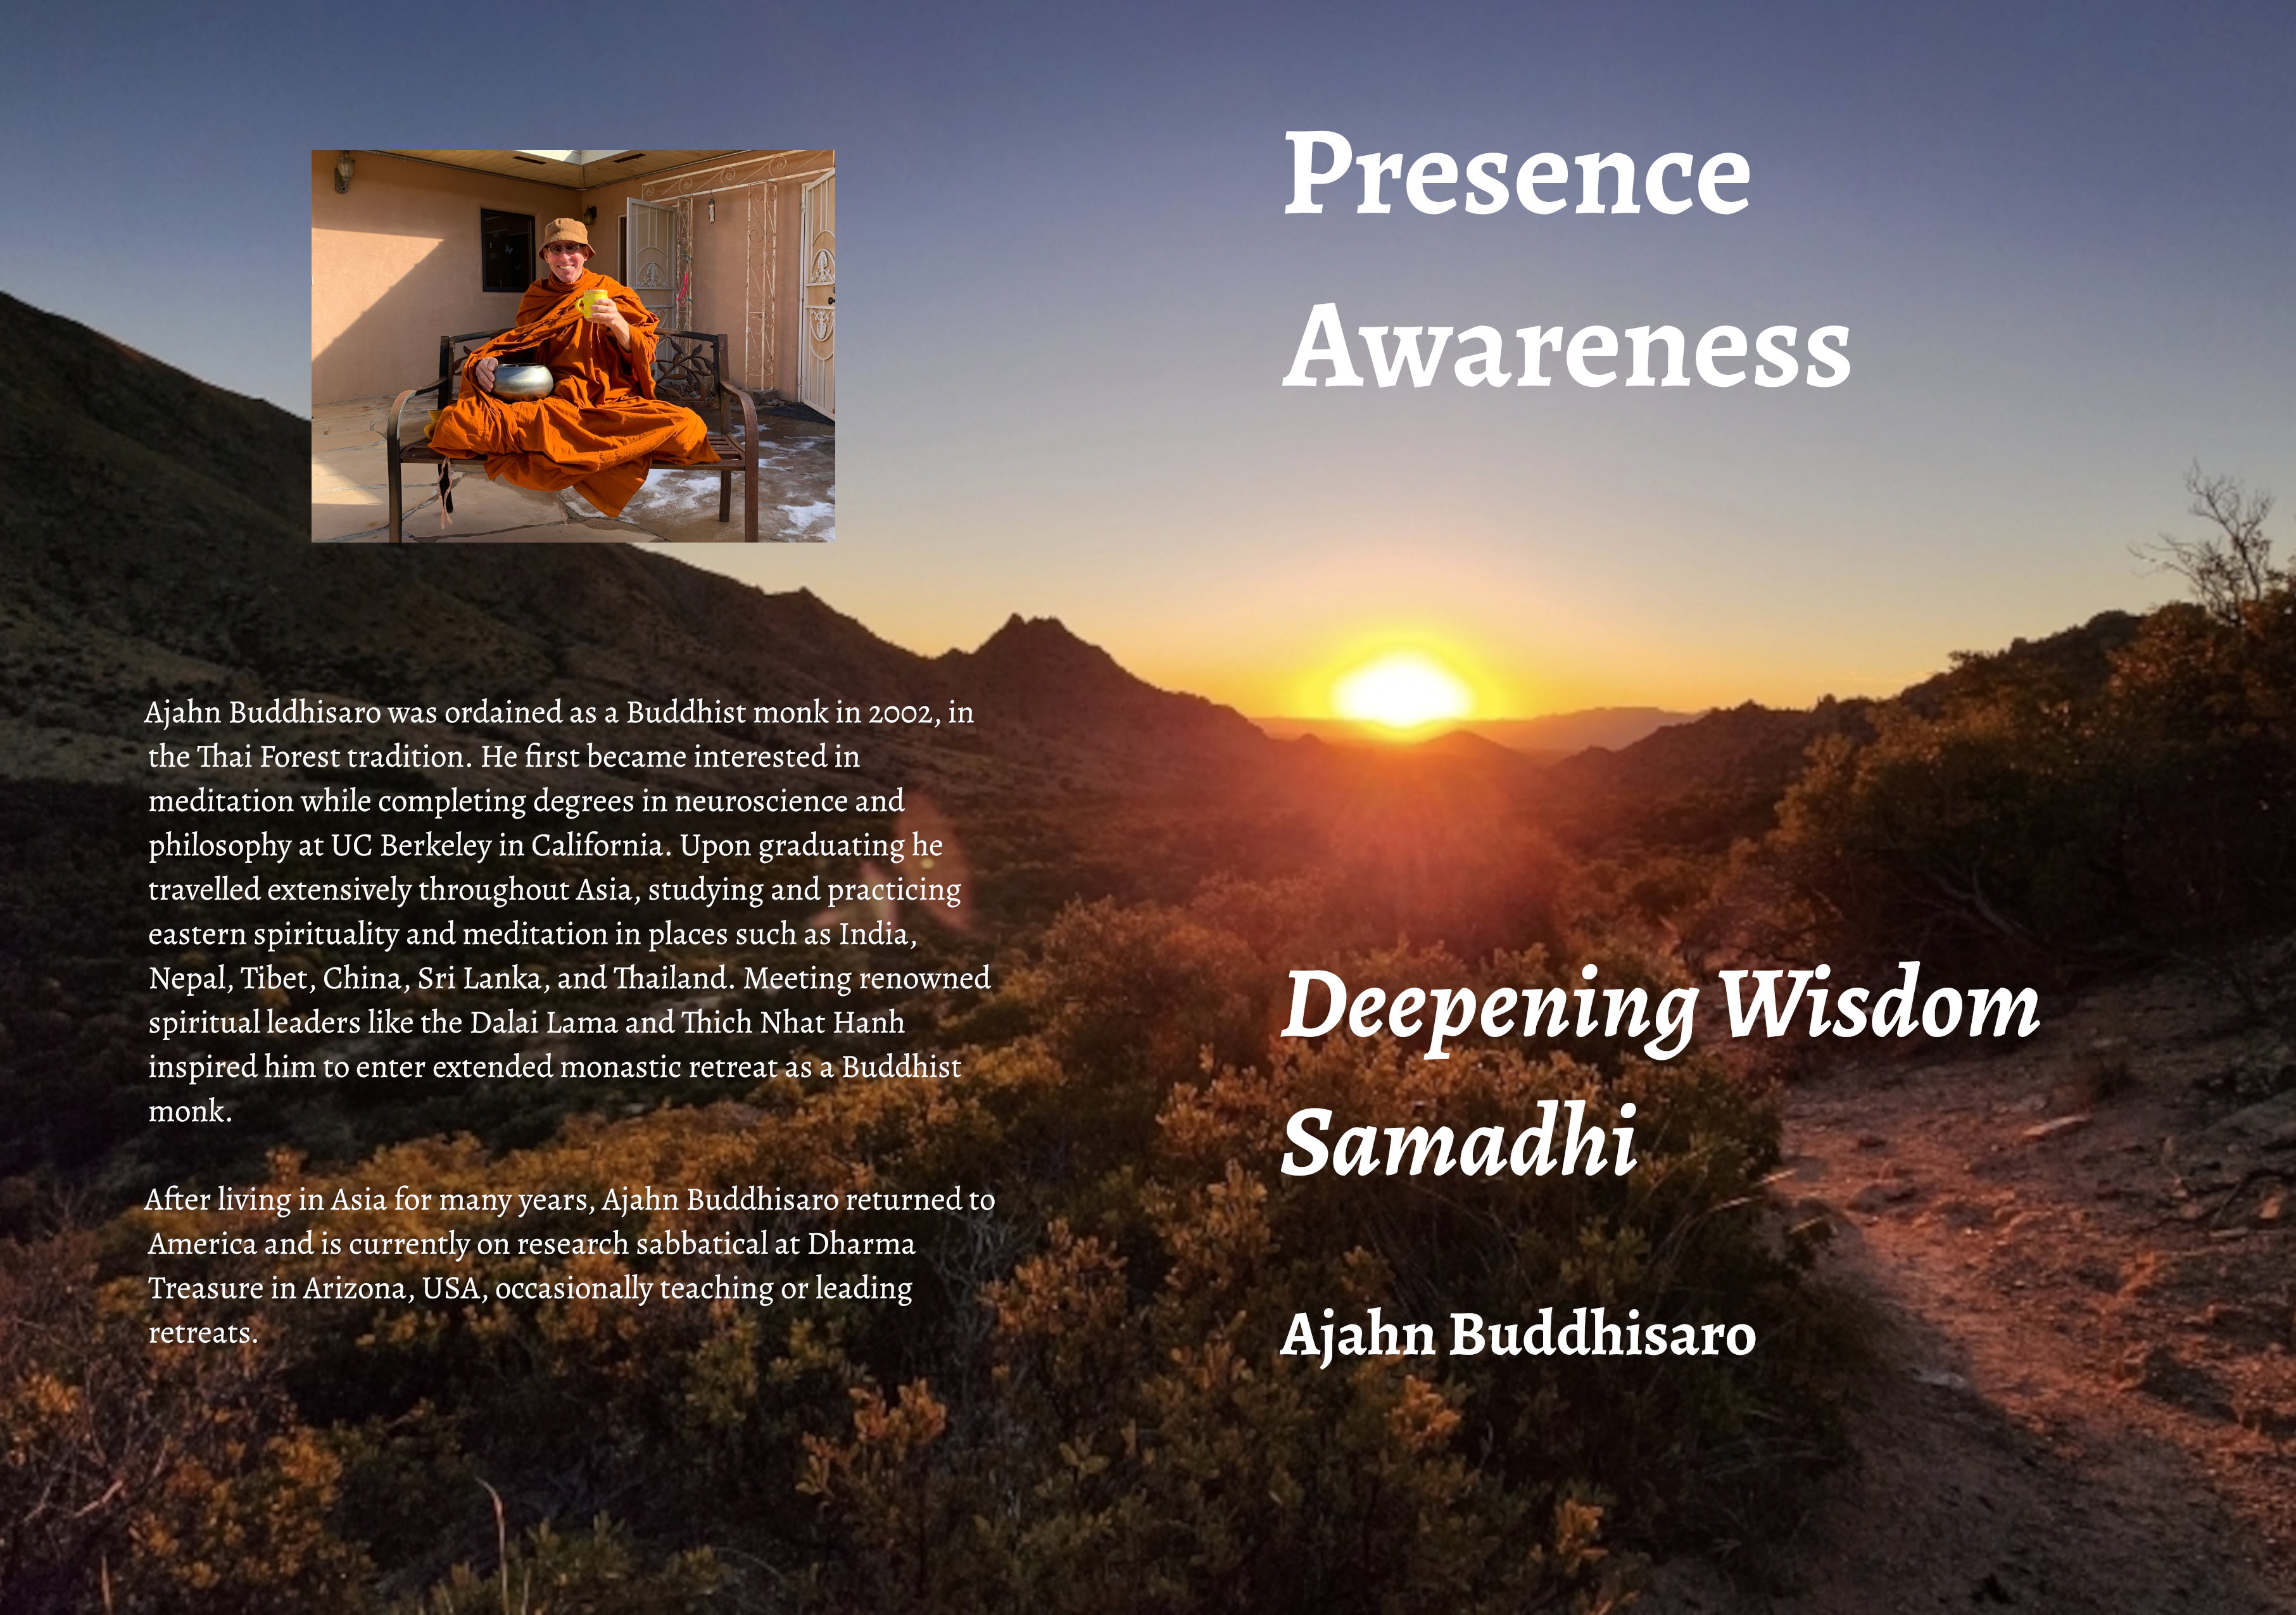
\includegraphics{cover.png}

\end{document}
